% This is file `elsarticle-template-1-num.tex',
%%
%% Copyright 2009 Elsevier Ltd
%%
%% This file is part of the 'Elsarticle Bundle'.
%% ---------------------------------------------
%%
%% It may be distributed under the conditions of the LaTeX Project Public
%% License, either version 1.2 of this license or (at your option) any
%% later version.  The latest version of this license is in
%%    http://www.latex-project.org/lppl.txt
%% and version 1.2 or later is part of all distributions of LaTeX
%% version 1999/12/01 or later.
%%
%% The list of all files belonging to the 'Elsarticle Bundle' is
%% given in the file `manifest.txt'.
%%
%% Template article for Elsevier's document class `elsarticle'
%% with numbered style bibliographic references
%%
%% $Id: elsarticle-template-1-num.tex 149 2009-10-08 05:01:15Z rishi $
%% $URL: http://lenova.river-valley.com/svn/elsbst/trunk/elsarticle-template-1-num.tex $
%%
\documentclass[preprint,12pt]{elsarticle}

%% Use the option review to obtain double line spacing
%% \documentclass[preprint,review,12pt]{elsarticle}

%% Use the options 1p,twocolumn; 3p; 3p,twocolumn; 5p; or 5p,twocolumn
%% for a journal layout:
%% \documentclass[final,1p,times]{elsarticle}
%% \documentclass[final,1p,times,twocolumn]{elsarticle}
%% \documentclass[final,3p,times]{elsarticle}
%% \documentclass[final,3p,times,twocolumn]{elsarticle}
%% \documentclass[final,5p,times]{elsarticle}
%% \documentclass[final,5p,times,twocolumn]{elsarticle}

%% if you use PostScript figures in your article
%% use the graphics package for simple commands
\usepackage{graphics}
%% or use the graphicx package for more complicated commands
\usepackage{graphicx}
%% or use the epsfig package if you prefer to use the old commands
\usepackage{epsfig}
%% Package for hyperlighting references
\usepackage{hyperref}
\hypersetup{hidelinks,colorlinks,breaklinks=true,urlcolor=color2,citecolor=color1,linkcolor=color1,bookmarksopen=false,pdftitle={Title},pdfauthor={Author}}
%% The amssymb package provides various useful mathematical symbols
\usepackage{amssymb}
%% The amsthm package provides extended theorem environments
\usepackage{amsthm}
\usepackage{amsfonts}
\usepackage{xcolor}
\usepackage{epstopdf}%adiciona imagens em formato eps no pdf.
\usepackage{subfig}%cria ambientes de multifiguras
\usepackage{float}
\usepackage{dblfloatfix}
\usepackage{blindtext} 
\usepackage{tikz}%pacote para fazer fluxogramas
\usetikzlibrary{calc,trees,positioning,arrows,chains,shapes.geometric,decorations.pathreplacing,decorations.pathmorphing,shapes,matrix,shapes.symbols}

\tikzset{
	>=stealth',
	punktchain/.style={
		rectangle,
		rounded corners,
		% fill=black!10,
		draw=black, very thick,
		text width=10em,
		minimum height=3em,
		text centered,
		on chain},
	line/.style={draw, thick, <-},
	element/.style={
		tape,
		top color=white,
		bottom color=blue!50!black!60!,
		minimum width=8em,
		draw=blue!40!black!90, very thick,
		text width=10em,
		minimum height=3.5em,
		text centered,
		on chain},
	every join/.style={->, thick,shorten >=1pt},
	decoration={brace},
	tuborg/.style={decorate},
	tubnode/.style={midway, right=2pt},
}

\tikzset{basic/.style={draw,fill=blue!50!green!20,
		text badly centered,minimum width=3em}}
\tikzset{input/.style={basic,circle}}
\tikzset{weights/.style={basic,rectangle,minimum width=2em}}
\tikzset{functions/.style={basic,circle,fill=blue!50!green!20}}
\newcommand{\addsymbol}{\draw[thick] (0.5em,0.5em) -- (0,0.5em) --
	(0,-0.5em) --  (-0.5em,-0.5em)
	(0em,0.75em) -- (0em,-0.75em)
	(0.75em,0em) -- (-0.75em,0em);}

\usetikzlibrary{positioning}

\tikzset{basic/.style={draw,fill=blue!20,text width=1em,text badly centered}}
\tikzset{input/.style={basic,circle}}
\tikzset{weights/.style={basic,rectangle}}
\tikzset{functions/.style={basic,circle,fill=blue!10}}

\usepackage{indentfirst}
\usepackage{multicol}
\usepackage{mathptmx}
\usepackage{xspace}
\usepackage{amsmath}
\usepackage{smartdiagram}

\usepackage[portuguese,english,brazil]{babel}

%% The lineno packages adds line numbers. Start line numbering with
%% \begin{linenumbers}, end it with \end{linenumbers}. Or switch it on
%% for the whole article with \linenumbers after \end{frontmatter}.
\usepackage{lineno}



%The Xwatermark is a package for write watermarks

\usepackage{xwatermark}

%% natbib.sty is loaded by default. However, natbib options can be
%% provided with \biboptions{...} command. Following options are
%% valid:

%%   round  -  round parentheses are used (default)
%%   square -  square brackets are used   [option]
%%   curly  -  curly braces are used      {option}
%%   angle  -  angle brackets are used    <option>
%%   semicolon  -  multiple citations separated by semi-colon
%%   colon  - same as semicolon, an earlier confusion
%%   comma  -  separated by comma
%%   numbers-  selects numerical citations
%%   super  -  numerical citations as superscripts
%%   sort   -  sorts multiple citations according to order in ref. list
%%   sort&compress   -  like sort, but also compresses numerical citations
%%   compress - compresses without sorting
%%
\biboptions{comma,round}

% \biboptions{}

\newwatermark[allpages,angle=60,scale=4,color=blue!8,xpos=-10pt,ypos=10pt]{D R A F T }

\journal{Journal of Applied Geophysics}

\begin{document}

\begin{frontmatter}

%% Title, authors and addresses

%% use the tnoteref command within \title for footnotes;
%% use the tnotetext command for the associated footnote;
%% use the fnref command within \author or \address for footnotes;
%% use the fntext command for the associated footnote;
%% use the corref command within \author for corresponding author footnotes;
%% use the cortext command for the associated footnote;
%% use the ead command for the email address,
%% and the form \ead[url] for the home page:
%%
 %\title{Title\tnoteref{label1}}
 %\tnotetext[label1]{Corresponding author}
 \author{Carreira,V. R. \corref{cor1}\fnref{label1}}
 \ead{victorcarreira@on.br}
 \ead{cosme@on.br}
 \ead{rodrigobijani@gmail.com}
 \ead[url]{www.on.br}
 %\fntext[label1]{Ponte-Neto, C. F.}
 %\cortext[cor1]{}
 %\address{Address\fnref{label3}}
 %\fntext[label2]{Bijani, R.}

%\title{A multi noisy rock data detection in a artificial intelligence context using well log data in Paran\'a Sedimentary Basin, South Portion of Brazil.}
\title{A comparison of three different artificial intelligence methods for detection of rock units: Application on well log data in Paran\'a sedimentary basin, South Brazil.}

%% use optional labels to link authors explicitly to addresses:
\author[label1]{Ponte-Neto, C. F. \corref{cor1}}
\address[label1]{Coordenacao de Geof\'isica, Observat\'orio Nacional (ON-MCTIC), Rio de Janeiro, Brasil}
\author[label2]{Bijani, R.}
\address[label2]{Departamento de Geologia e Geof\'isica, Universidade Federal Fluminense (UFF), Niter\'oi, Brasil}

\begin{abstract}
Refazer do zero a partir dos resultados e da abordagem deste trabalho.


\end{abstract}

\begin{keyword}
Paran\'a Sedimentary Basin \sep Artificial Intelligence \sep Well-log data \sep Identification of Lithologies 
%% keywords here, in the form: keyword \sep keyword

%% MSC codes here, in the form: \MSC code \sep code
%% or \MSC[2008] code \sep code (2000 is the default)

\end{keyword}

\end{frontmatter}

%%
%% Start line numbering here if you want
%%
\linenumbers

%% main text
\section{Introduction}
\label{sec:intro}

Machine learning problems is divided into two main groups of problems. One that deals with regression problems such as minimization and inversion. And another group that deals with classification.  Machine learning field approaches the creation of computer program's that have the capability of automatically improve themselves through experience \citep{Michie1994,MacKay2005}. 


Classification techniques such as Euclidean and Mahalanobis similarity measurements are considered classical machine learning methods.  Those similarity measurements are referred to as distance attributes \citep{Deza2016}. Euclidean classifiers include a calculation of a centroid on the space of attributes. While the Mahalanobis takes into consideration the shape of attributes space. Both techniques are capable of making identification of geological cyclic in data \citep{Bergen2019}.


A Self-Organizing Map (SOM) is inspired by neural cortex \citep{Kohonen1989}. A SOM algorithm uses a general learning paradigms called unsupervised learning and is based on a network fully connected \citep{Haykin2001}. This geometric arrangement is an oriented graph, whose vertices are the fundamental units know as artificial neurons and the edges are weights governing the interactions among neurons. Those artificial neurons change their weights as iterations go on. Categorized as an unsupervised-competitive learning algorithm SOMs are excellent data-exploring tool. It projects high-dimension patterns onto a low-dimensional topology map \citep{Chaudhary2014}. The neuron activation is a function of distance between neuron weight and input data. The so called winner neuron is the graph node's that have the minimum distance value, in euclidean terms. Once a winner neuron is selected it alters the weights of the surrounding neurons obeying a neighbor function rule. An iteration processes of neurons weights recalculation it goes on until it reaches a total epoch time limit, reflecting the data distribution. An important characteristic of the SOM network is that it preserves the topology of the input data by assigning each datum to a neuron having the highest similarity, in other words, having the smallest euclidean distance. And the data with similar attributes are mapped into adjacent neurons \citep{kohonen2013}. 


\citet{Carneiro2012} uses SOM to infer how clustering outcrops rock units, in Anapu-Tuer\^e province inside the Amazon region, using aerogeophysical data and spatial analysis. \citet{Pastukhov2016} uses kohonen-SOM to train a multi-layer perceptron (MLP). This strategy creates new models for data clustering. This clustering factor allows to create a representative sample that contains unique sets of attributes used in validation and training tests. \citet{Sahoo2017} uses a hybrid SOM with Genetic Algorithm (GA) to characterizing lithology in groundwater basins using well log data. Concerning only metamorphic rocks such as orthogneiss, paragneiss, eclogite, amphibolite and ultramafic rocks \citet{Konate2015} compare classification of SOMs result with feed-forward neural network (FFNN) using t-test to guide the classification decision. This study shows that SOMs are comparable to FFNNs in classifying lithology in drilling research.   

\citet{Valentin2019} relates borehole images with petrophysical properties characterizing reservoir rocks in a facies scale using deep residual convolutional neural networks (ResNetRock). \citet{Goncalves2017} uses a series of classification algorithms such as k-nearest neighbors, Naive Bayes, Random Forest, Sequential minimal optimization and Multi Layer Percetron to identify carbonate rocks based on relaxation times in Nuclear Magnetic Resonance logging data. 

Machine learning and artificial intelligence in geophysics is divided according \citet{Poulton2002} into two main period. First period, during the 80ths geoscientists were running experiments to underscore what kind responses machine learning and artificial intelligence models can do to make predictions in both fields of regression and classification problems mainly with synthetic data. During the late 90ths and beginning of the year 2000, geoscientists were working basically with real data to make predictions. Nowadays, geocientists are returning to simulations to understand what problems could affect real world problems. \citet{Akinnikawe2018} uses photoelectric effect information to generate synthetic logs. \citet{Zhang2016} uses synthetic data to training ANN's to make images predictions. \citet{Rolon2009,Rolon2005} generates a synthetic Magnetic Resonance Imaging (MRI) logs using conventional well logs such as Spontaneous Potential, Gamma Ray, Caliper, and Resistivity for four wells located in East Texas, Gulf of Mexico, Utah, and New Mexico.       



%From a geophysical perspective, two big problems rise during a drill performance. Firstly is recovery lithological data in relation to depth. Secondly is manage a target horizon e.g., in a petroleum system, a source rock such as a shale rich in organic matter or, even thought, a reservoir rock like sandstone (conventional petroleum systems) or basalt or shale (non-conventional petroleum system).


This article presents the best comparative methodology for tree classifiers that solves the first problem concerning lithological recovery along a geologic normal fault. Two statistical classifiers and one neural network (SOM) that solves the first problem in a well log data set in a synthetic sedimentary Basin with different noisy data. And a real application for a general overview and identification for sedimentary rocks in a drill core in Paran\'a Sedimentary Basin.  

\section{Geological Setting}
\label{sec:GeoSet}
Parana Basin (Fig. \ref{fig:Geomap}) is composed by a sedimentary and a magmatic package with a maximum thickness around 7,000 m, which geographically coincides with the syneclise structural center and the channel of the Parana River \citep{Milani1998,Milani2008}. The stratigraphy record of Parana Basin is divided into six broad scale units or super-sequences \citep{Vail_1977} as rocky packages with time intervals of a few tens of millions of years of duration and enveloped by surfaces of inter-regional character of nonconformity: Rio Ivai (Ordovician-Silurian), Parana (Devonian), Gondwana I (Carboniferous-Eotriassic), Gondwana II (Meso to Neotriassic), Gondwana III (Neojurassic-Eocretaceous) and Bauru (Neocretaceous). The first three supersequences are represented by sedimentary sequences that define transgressive and regressive cycles linked to fluctuations in relative sea level during the Paleozoic, while the rest correspond to continental sediment packages with associated igneous rocks. The formal lithostratigraphy units, whichever are the groups, formations and members commonly used in describing the spatial arrangement of the basin strata, are inserted as individualized elements in the regional scale aloestratigraphic framework \citep{Vidotti_1998,milani_outline_1999}

\begin{figure*}[!htb]
\centering
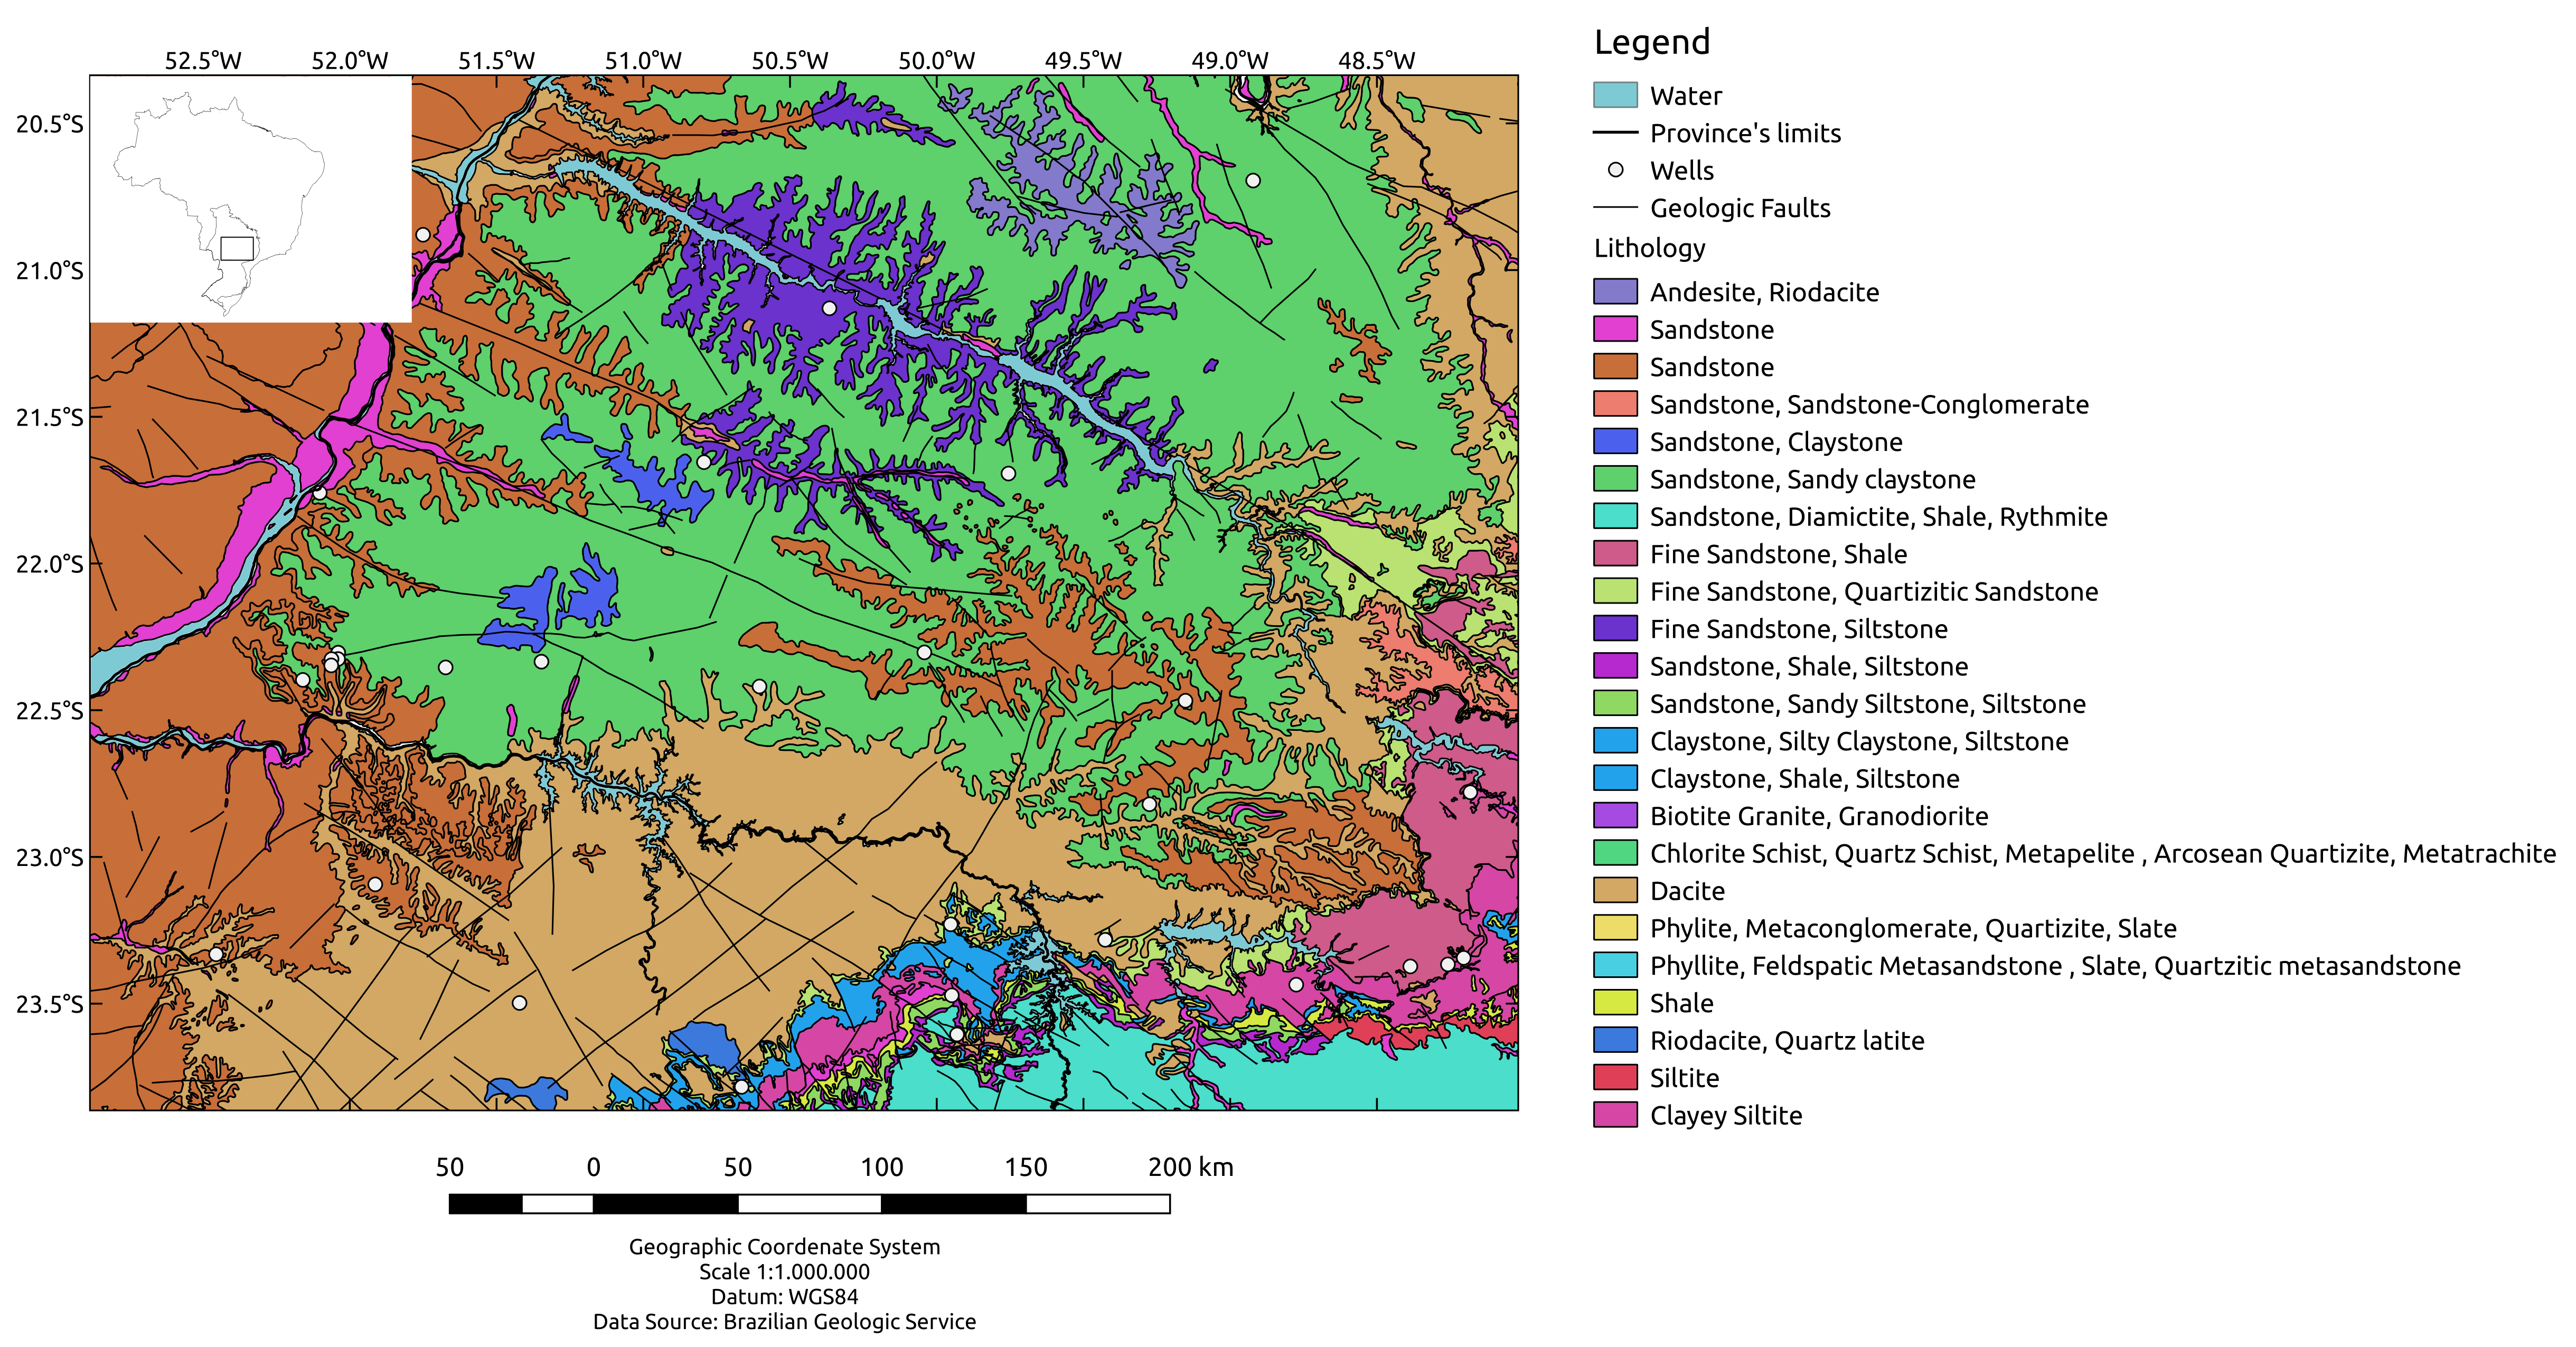
\includegraphics[scale=0.4]{imagens/geologicwells.png}
\caption{Geologic map.  The white board shows the geopolytical limits of Brazil and the geologic boarder of Paran\'a Sedimentary Basin inside brazilian territory. The black square indicates the studied region. The amplified map shows the lithological spatial distribution of rocks in the central part of Paran\'a Sedimentary Basin, geologic faults and localization of the drilling data using in this work.}
\label{fig:Geomap}
\end{figure*}


\section{Methods and applications}
\label{sec:MetAp}
The methodology proposed in this paper is based on the evaluation of three different artificial intelligence methods in classifying rock types from well log data. To achieve this goal, Euclidean and Mahalanobis multivariate statistic methods are considered. In our application, both belong to supervised classification scheme, which correlates new data points and labelled data by means of metrics in data space. (REFERENCIAS SUPERVISIONADOS). Additionally, a Self-Organizing Map (SOM) with discrete neighboring function is implemented. The latter is a neural network algorithm based on Penfield's homunculus \citep{ritter1989,Haykin2001,kohonen2013} and belongs to unsupervised classification scheme, which comprises the clustering of unlabelled data \citep{fankhauser2005, nabney2003, weinberger2009,chatpatanasiri2010,Deza2016}. Each method is briefly described in the following sections.      

\subsection{Euclidean Classifier - EC}
\label{sub:EC}
Consider a multidimensional data set, in matrix notation, as 
\begin{equation}
\textbf{$\textbf{X}$} =
\begin{vmatrix} 
x_{11} & x_{12} & x_{13} & \hdots  & x_{1M} \\
x_{21} & x_{22} & x_{23} & \hdots  & x_{2M} \\
x_{31} & x_{32} & x_{33} & \hdots  & x_{3M} \\
\vdots & \vdots & \vdots & \ddots  &\vdots  \\
x_{N1} & x_{N2} & x_{N3} & \hdots  & x_{NM}
\end{vmatrix},
\label{eq:multidata}
\end{equation}
where $N$ states for the data sampling (i.e., lines of matrix $\mathbf{X}$) and $M$ for the different number of data types (i.e., columns of matrix $\mathbf{X}$). 
The Euclidean classifier ($EC$) is a statistical clustering method that uses the concept of a distance function between two points in Euclidean space. In matrix formulation for multivariate data set, the $EC$ can be formulated as
\begin{equation}
E(\mathbf{X})= \frac{1}{N} || (\mathbf{X} - \bar{\mathbf{\mu}}_i)^{T} \mathbf{I} ~ (\mathbf{X} - \bar{\mu}_{i}) ||_2, ~~~i=1,\hdots, \kappa
\label{eq:EC}
\end{equation}
where $|| . ||_2$ states for the L-2 norm, superfix $^T$ denotes matrix transpose, $\mathbf{X}$ is the input data to be classified, named herein as classifying data, $\mathbf{I}$ is an identity matrix of order $M$, $\kappa$ is the total number of clusters and $\bar{\mu}_i$ is the $i$-th mean value (i.e., the $i$-th cluster) of each data type comprising a set of training data. The minimization of Equation \ref{eq:EC} accomplishes the optimal location for $\bar{\mu}_i$. In the $EC$ algorithm, the observed data is compared to the prior clusters, defined by its nearest mean. Consequently, each data point is linked to the cluster with the nearest vector \citep{nabney2003, karmakar2018}.    

\subsection{Mahalanobis Classifier - MC}
\label{sub:MC}
Mathematically, Mahalanobis sample distance, called herein as Mahalanobis Classifier ($MC$) can be defined as:
\begin{equation}
M_{i}(\mathbf{X})=|| (\mathbf{X}-\bar{\mu}_{i})^{T} \mathbf{C}_{i}^{-1}(\mathbf{X}-\bar{\mu}_{i}) ||_2,
\label{eq:maha}
\end{equation}
where $\mathbf{C}_i^{-1}$ is the inverse of covariance matrix of the $i$-the class (or cluster) and $\bar{\mu}_i$ is the corresponding class mean. The $\mathbf{C}_i$  can be expressed by the following expression:
\begin{equation}
\textbf{C}_{i}=\frac{1}{N_{k}}\sum_{k=1}^{N_k}(\textbf{X}_i-\bar{\mu}_{k})(\textbf{X}_i-\bar{\mu}_{k})^{T},
\label{eq:covC}
\end{equation}
where $N_k$ is the number of training samples in the $k$-th cluster. If the covariance matrix $\textbf{C}_{i}$ is identical to the identity matrix $\textbf{I}$, then $MC$ and $EC$ are equivalent methods. 
 
Often in practice, we are interested in measuring and then summarizing the differences between groups, here  A common assumption is to take the p-dimensional random vector X as having the same variation about its mean within either group. Then the difference between the groups can be considered in terms of the -difference between the mean vectors of X, in each group relative to the common within-group variation.

\subsection{Self-Organizing Map - SOM}
\label{sub:SOM}
SOM are machine learning types composed by oriented graphs that are distributed on a hyperplane inside a hyperspace of features. Features are the physical properties that are correlated with a specific type of rock. The identification process is based on redundancy of patterns. A toroid geometry is adopted here for the SOM with $400$ neurons. 

Let it be \textbf{R} the whole training dataset composed by all log data. \textbf{W} is weight matrix. $i$ and $j$ are index representing positions in the graph. Vector \textbf{x} is composed of physical properties from the training data with dimension $n$, where $n$ is the number of data measured that composite the \textbf{R} matrix. \textbf{x} is related to a neuron with a $\textbf{W}_{i,j}$ weight matrix, as follows:

i an j are the indexes of each neuron. In a euclidean meaning a winner neuron starts the actualization process as follows

\begin{equation}
     |\textbf{W}_{ij} \ast - x_{ij}| \leq |\textbf{W}_{ij} - x_{ij}| 
\end{equation}

Where $\ast$ indicates the winner neuron. 


The iterative process goes as follows

\begin{equation}
 \Delta \textbf{W}  = \eta \Lambda (ij,ij\ast) (x - w_{ij})
\end{equation}


where $\eta$ is the learning rate. In this work, the learning rate is defined as

\begin{equation}
  \eta = 1 - \frac{t}{T}
\end{equation}

t is an specific iteration and T is the total number of iteractions or epoch time. 



%\begin{displaymath}
% \mathbf{R}=\left(\begin{array}{r}
%   x_{1}\\
%   x_{2}\\
%   x_{3}\\
%  \vdots \\
%   x_{m}
% \end{array}\right)
% \end{displaymath}

%\begin{eqnarray}
%d(t)= \sqrt{\sum^{n}_{i=1}[x(t)-w_{i,j}(t)]^{2}}\\ 
%(j = {1,..,m}), \nonumber
%\label{eq1}
%\end{eqnarray}

 where $t$ is the number of iterations, $x(t)$ is an element of \textbf{X} and $d(t)$ is the metric. The lowest value of $d(t)$ defines the best neuron for a specific attribute.

\subsection{WELL LOGGING DATA}
\label{sub:WLG}
For a reliable prediction of rock types in a well, log data are strictly necessary. $EC$, $MC$ and $SOM$ methods are dependent on input log data, which we referred here as training data. In this work, each column of multidimensional input data $\mathbf{X}$ is composed by density log ($RHOB$ in $g/cm^3$), gamma-ray log ($GR$ in $API$), spontaneous potential log ($SP$ in $mV$) and sonic log ($DT$ in $\mu s/ m$). The training data should be consistent with the associated rock unit to guarantee a reliable application of the proposed methodology. To achieve this purpose, we design a controlled geological cross section similar to some structures interpreted in Paran\'a sedimentary Basin, as explained in the following section.

%\begin{figure*}[h]
%	\centering
%	\includegraphics[scale=1.5]{imagens/T1130118.eps}
%	\caption{Synthetic training well T$1$. The normal fault was created by four divisions on the range of the normal fault, decreasing the amount of conglomerate in comparison to crystalline basement. That behavior simulates a special kind of logging signature. }
%	\label{t1}
%\end{figure*}


\section{Synthetic Geological Scenario}
\label{sec:SynGeo}
To aim the scope of this work, we first design a synthetic geological scenario comprising a cross section of the Solim\~oes Sedimentary Basin in North Brazil, an intracratonic basin interpreted in \cite{Sal2008} (see Figure \ref{fig:Model}). Horts, Grabens, normal and reverse faults are the major geologic structures in Solim\~oes sedimentary basin, which are also encountered in Paran\'a basin \cite{Zanotto_1993, Zalan2007}.  
Additionally, a zoom box of two normal faults simulating a contact zone of two group of rocks conglomerate-crystalline and shale 2-crystalline are also shown in Figure \ref{fig:Model}.

As can be seen in Figure \ref{fig:Model}, $T1$, $T2$, $T3$, $T4$, $T5$ are all training wells considered in our synthetic examples and $C1$, $C2$ and $C3$ are the classification wells. The synthetic log data is computed at a ratio of $0.01$ measure per meter, a compilation of literature information \citep{bassiouni1994} and real log data of Paran\'a basin provides physical property values for all rock units within the well, as can be seen in Table \ref{tab:Tab1}.  Once values of rock properties per lithotypes were compiled a well log data can be modeled. A well log data carries out variation of physical properties per depth. A synthetic well log data is modeled by calculating the standard deviation based on an average value of a single rock present in Table \ref{tab:Tab1}, plus a pseudoradom number. Pseudorandom number is a sortition taked by Gaussian distribution over the range between 0 and 1.   

For simulating the normal faults observed in wells $C1$ and $C3$, mixture law \citep{nery2013} involving two specific lithologies is considered. The law states that in a multicomposed systems each component volumetrically contributes for each component of the rock fraction plus each specific physical property elevated by a factor of $m$. Factor $m$ makes reference to a geometric distribution in a specific mixture. This work consider a linear distributions of each rock component ($m=1$). Let is be \textbf{R1} a set of properties that defines a specific rock $\textbf{R1}=[x_{1}^{1}, x_{2}^{1}, x_{3}^{1}, x_{4}^{1}]$ and \textbf{R2} a set of properties that defines another group of rock $\textbf{R2}=[x_{1}^{2}, x_{2}^{2}, x_{3}^{2}, x_{4}^{2}]$ a fault $\textbf{F}$ can be defined as

\begin{equation}
	F=[\phi \textbf{R1}^{m} + (1-\phi)\textbf{R2}^{m}]^{1/m}
	\label{misturelaw}
\end{equation}
      where $\phi$ is the fault declination and $m$ is the geometric distribution. For the linear case $m=1$ is considered to model a normal fault. $\textbf{R1}$ and $\textbf{R2}$ carry out the information about quantities of rock properties present in each mixture parts held in percentages after the rock name. To represent a mixture in a normal fault is considered here four equal parts in the squared area dominated by the fault. Wich  1/4 squared part brings the information of   
 

%(FOR EXAMPLE: TO REPRENT DE NORMAL FAULT SHONW IN FIGURE BAR ...) explicar aqui as falhas específicas e a terminilogia usada (co-ce 20, etc) fazer citação!!!.   

 
To generate the synthetic log data, four physical properties are considered: density ($RHOB$ - $g/cm^{3}$),  gamma-ray ($GR$ - $Ci/g$), spontaneous potential ($SP$ - $mV$), and sonic ($DT$ - $\mu s/ m$). Table \ref{tab:Tab1} illustrates all simulated property values, mostly extracted from literature \citep{bassiouni1994} and real log data of Para\'a basin. The sample rate for each log data is $0.01$ observation per meter and $5$\% Gaussian noise are added to the simulated log data. 

\begin{figure*}[!htb]
	\centering
	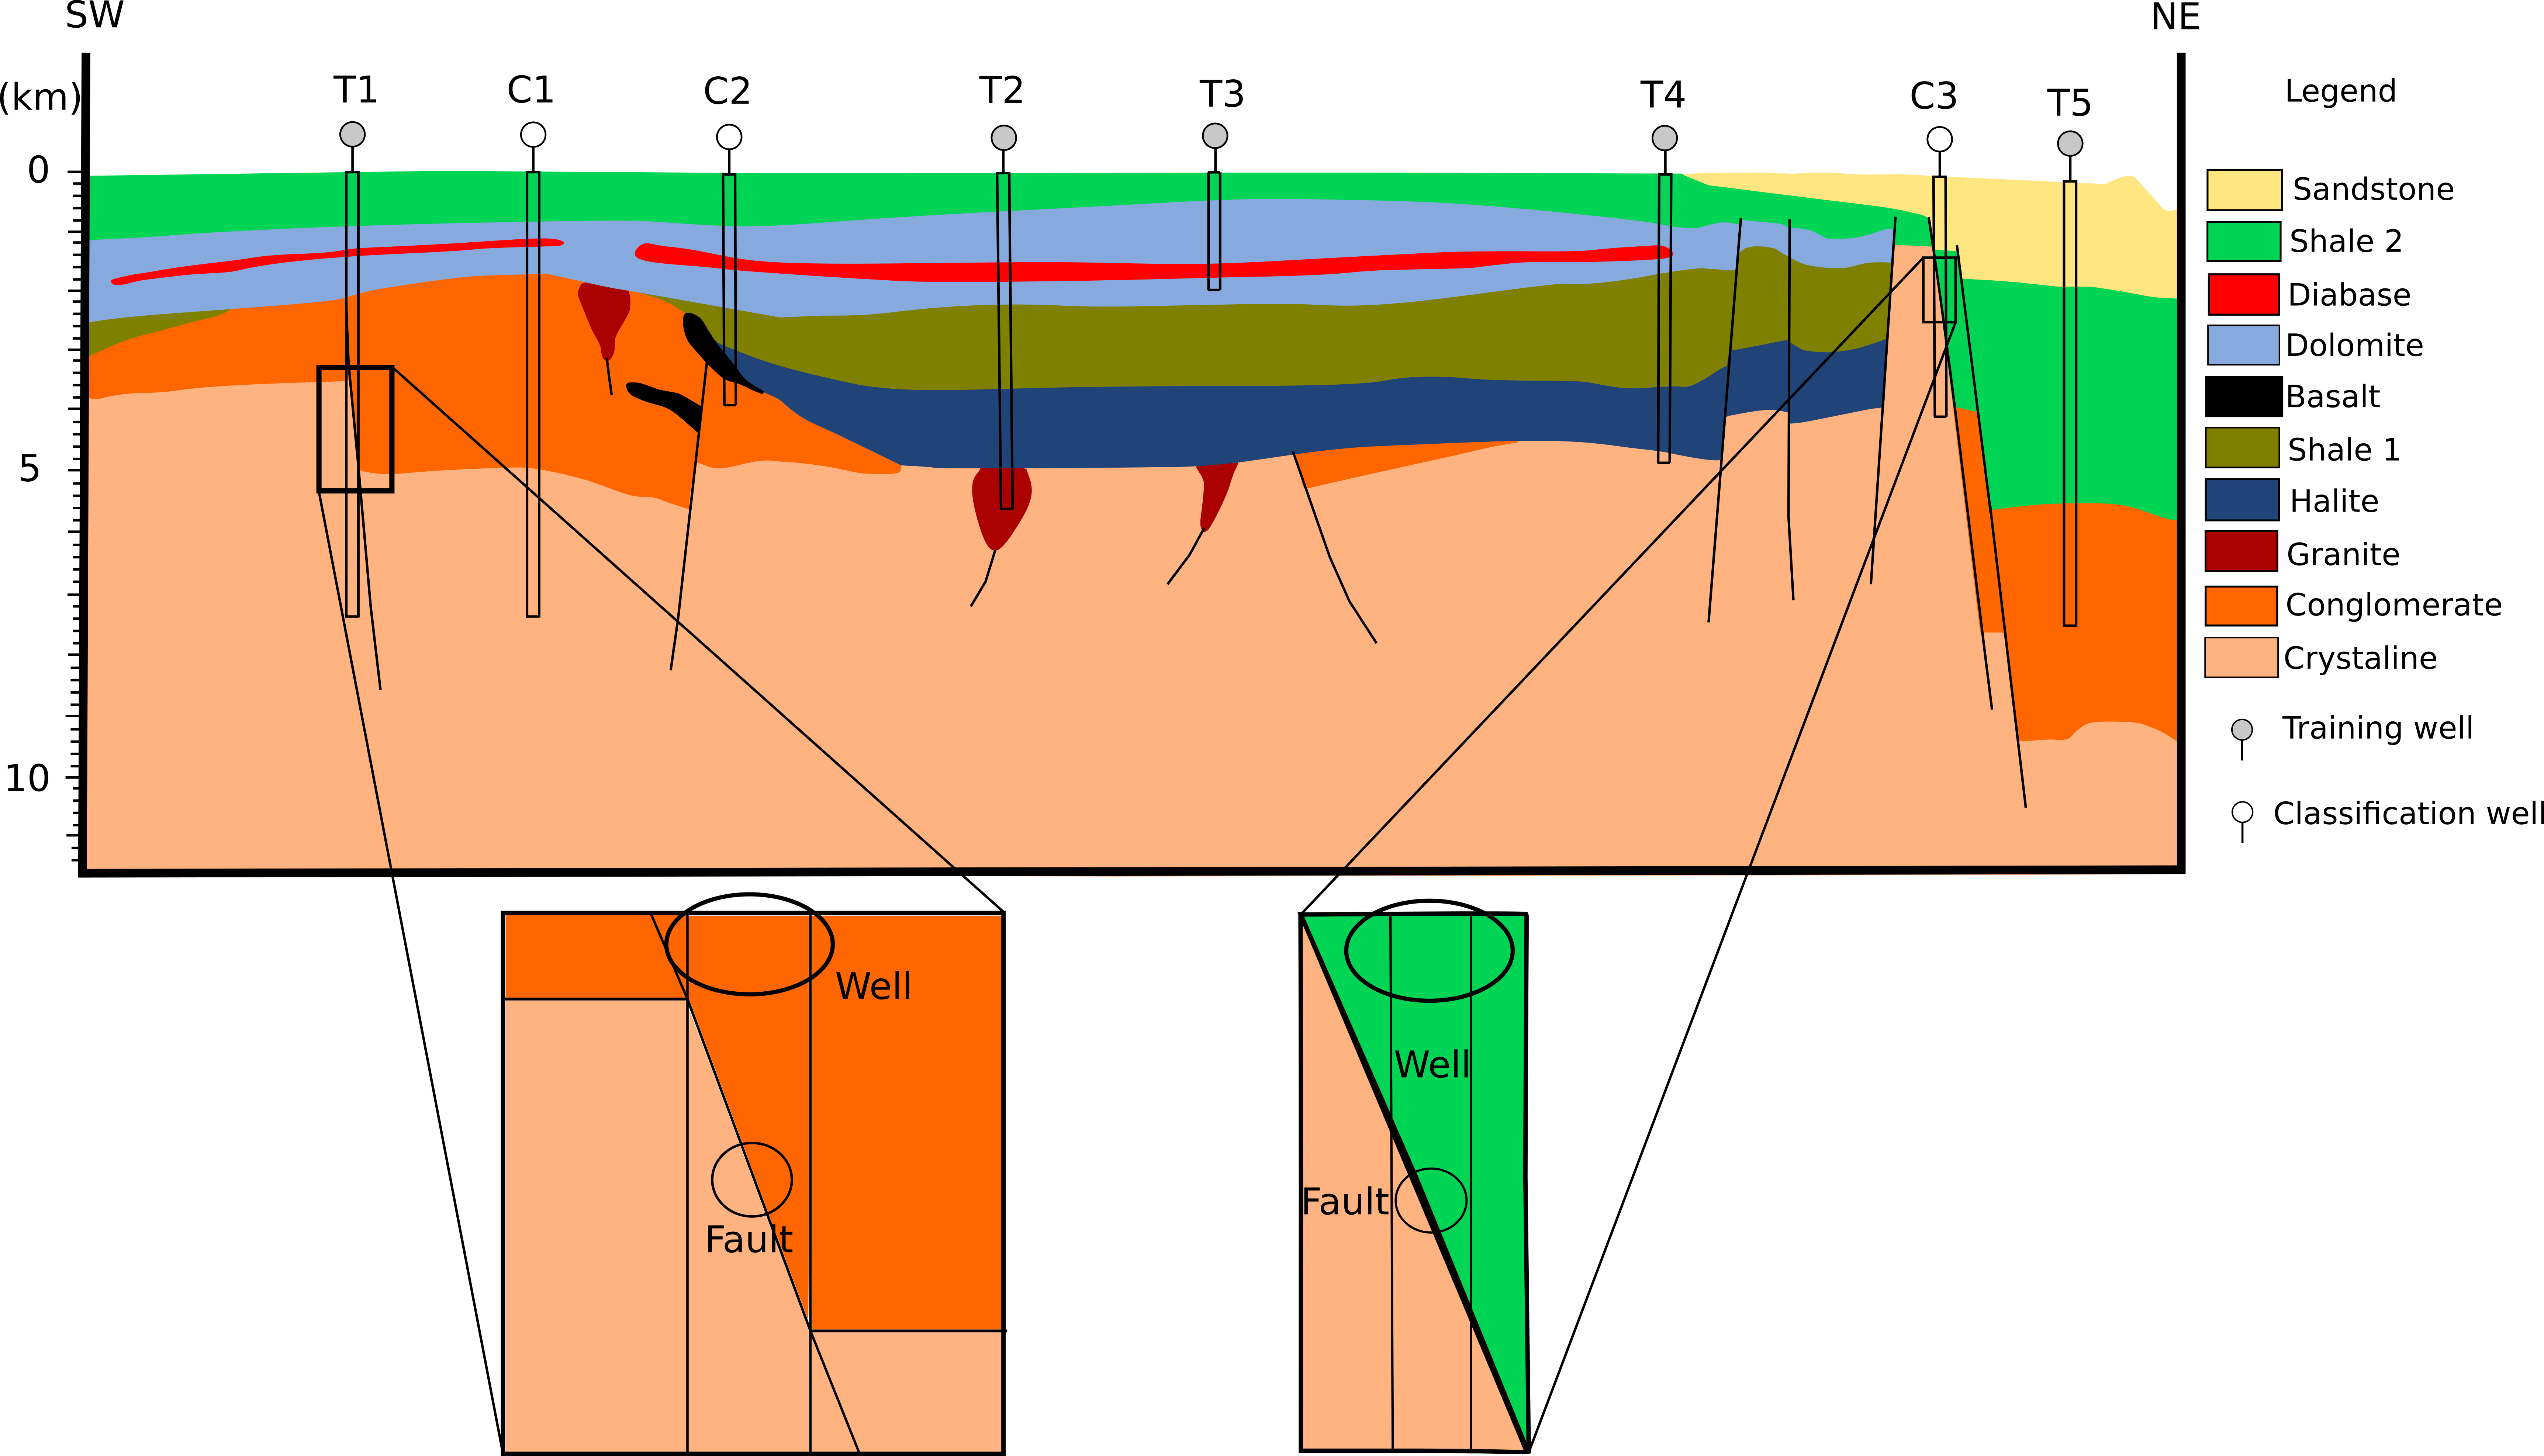
\includegraphics[scale=0.5]{imagens/Basin.png}
	\caption{The geologic section representing the on-shore syneclise sedimentary section by \cite{Sal2008}. Symbols T1, T2, T3, T4 and T5 comprise the synthetic wells used as training database. The classification wells are C1, C2, C3 respectively. The zoom box highlights two simulated normal faults involving Conglomerate and Crystalline, Shale 2 and Crystalline.}
	\label{fig:Model}
\end{figure*}

Two scenarios are proposed. First is a classic scenario when all lithotypes are present inside databank. It is represented by C1, C2 wells respectivelly. The second is non-classic scenario when a lithotype have no representativeness inside the databank. And it is represented by C3 and C4 wells respectively.  


\begin{table}[H]
	\centering
	\footnotesize
	\begin{tabular}{@{}ccccccccccc@{}}
		%\toprule
		Rock         &   $RHOB$   &    $GR$     &     $SP$   &    $DT$    &\\ %\midrule
		Conglomerate &  $2.30 \pm 0.046  $  &  $20.0 \pm 2.0$   &  $-40.0 \pm 4.0$ &   $110 \pm 11.0$   &\\
		Shale 2	     &  $2.48 \pm 0.049$  &  $110.0 \pm 11.0 $  &  $70.0 \pm 7.0$  &   $550 \pm 55.0$   &\\
		Dolomite     &  $2.52 \pm 0.05$  &  $40.0 \pm 4.0$   &  $-60.0 \pm 6.0$ &   $142 \pm 14.2$   &\\
		Diabase      &  $2.80 \pm 0.056$  &  $30.0 \pm 3.0$   &  $90.0 \pm 9.0$  &   $50 \pm 5.0$   &\\
		Crystalline  &  $2.75 \pm 0.055$  &  $40.0 \pm 4.0$    &  $70.0 \pm 7.0$  &   $55 \pm 5.5$    &\\
		Shale 1      &  $2.58 \pm 0.051$  &  $230.0 \pm 23.0$  &  $75.0 \pm 7.5$  &   $520 \pm 52.0$   &\\
		Halite       &  $2.16 \pm 0.043$  &  $11.0 \pm 1.1$   &  $6.0 \pm 0.6$   &   $216 \pm 21.6$  &\\
		Granite      &  $2.67 \pm 0.053$  &  $150.0 \pm 15.0$  &  $-60.0 \pm 6.0$ &   $68 \pm 6.8 $   &\\
		Sandstone    &  $2.31 \pm 0.046$  &  $20.0 \pm 2.0$   &  $120.0 \pm 12.0$ &   $170 \pm 17$   &\\
		Basalt       &  $2.87 \pm 0.057$  &  $15.0 \pm 1.5$   &  $50.0 \pm 5.0$  &   $65 \pm 6.5$   &\\ %\bottomrule
	\end{tabular}
	\caption{Rock-property values and the standard deviation of each rock unit for simulating the log data used in all synthetic cases. Shale 1 simulates a shale rock enriched by organic matter with high values of Gamma-ray. In opposition to the shale 2 that simulates rock shale poor in organic matter. }
	\label{tab:Tab1}
\end{table}

\subsection{Training database}
Figure \ref{fig:BD} shows all pair of cross plots for each rock unit and it properties within all training wells. In this case, the training wells, referred here in as the synthetic training database, show some important features about the distribution of log data in a discrete framework. From the histograms (on the diagonals of the pair plot) it can be seen that some variables contained overlap that would negatively affect model prediction. In RHOB histogram most of the normal distribution  have non-symmetric quantiles  and standard deviation of most of the rock types overlaps. In GR histogram standard deviation for shale 1 and shale 2, dolomite and halite, sandstone and conglomerate are clearly separated and symmetric quantiles. SP histogram have overlaps  for standards deviations of rock shale 2, shale 1, crystalline, and for dolomite and granite. Are clearly separated conglomerate, halite and dolomite. DT histogram indicates overlaps for shale 2 and shale 1 and relatively separation of all group of rocks.  


\begin{figure*}[!htb]
	\centering
	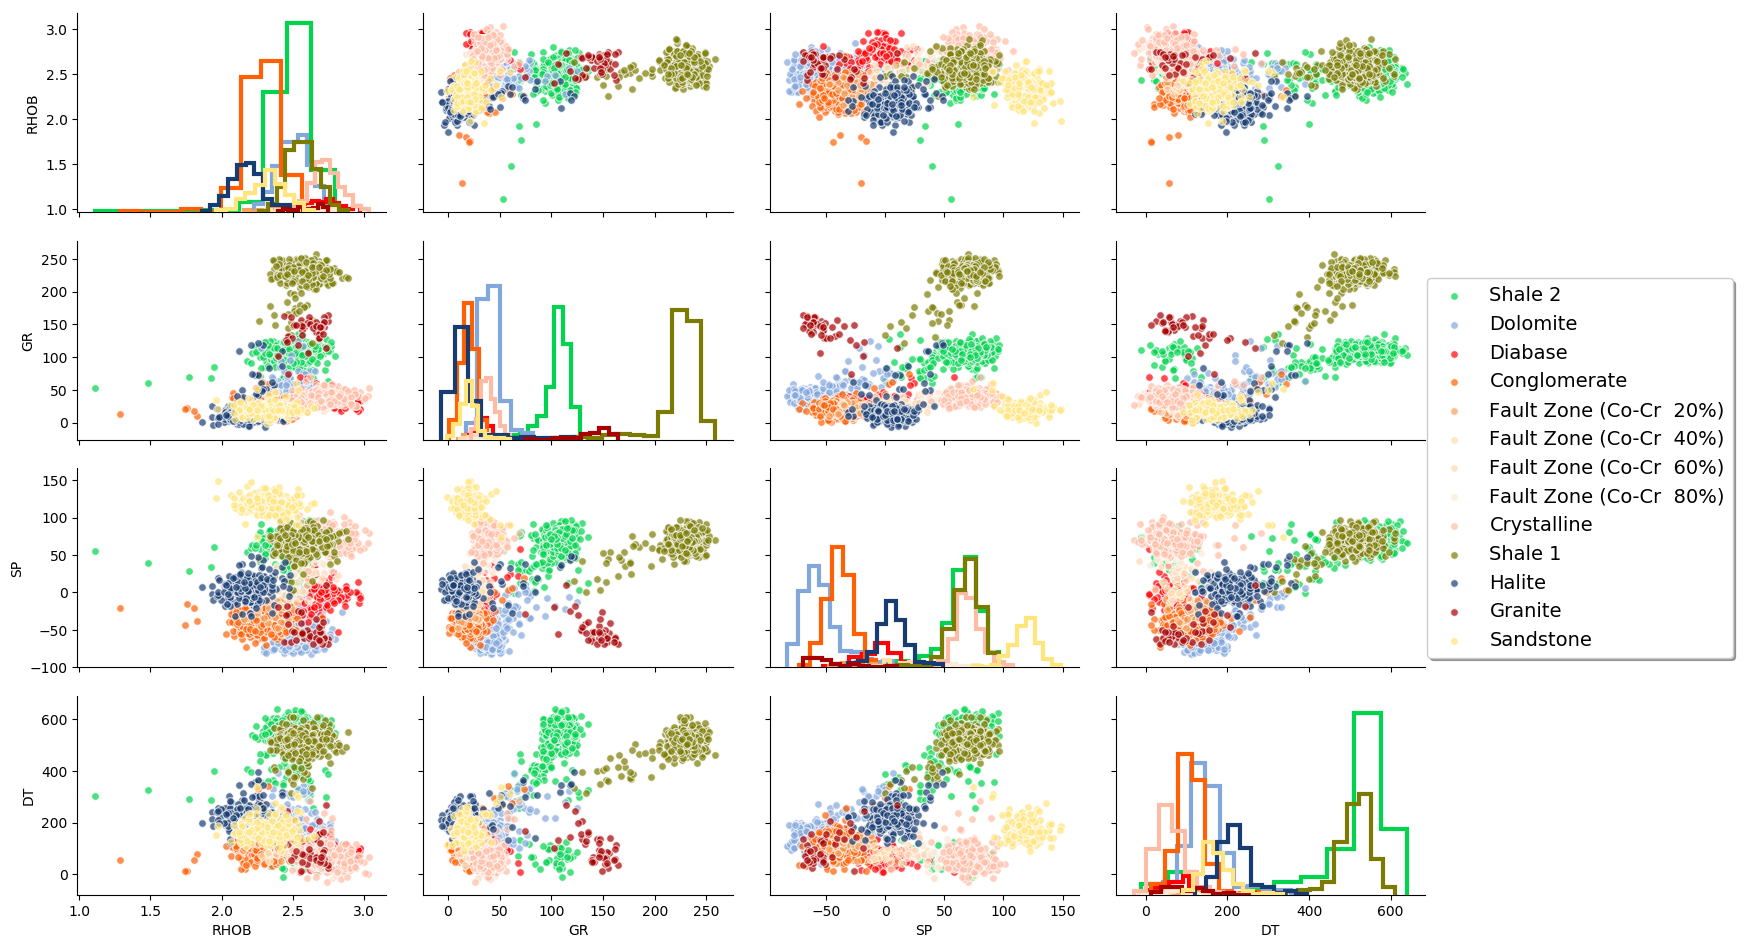
\includegraphics[scale=0.38]{imagens/BDsintetico_convolvido.png}
	\caption{Dispersion analysis for the training database composed by wells $T1$, $T2$, $T3$, $T4$ and $T5$ (see Figure \ref{fig:Model}). Legend identify all rock units comprising the training database.}
	\label{fig:BD}
\end{figure*}



The pair plot for GR and DT indicates some outliers that observable by two different clusters among shale 2. A filter was not applied in the channel GR because it is expected high range of values of rock formation in general.  The cross plots between profiles RHOB $ \times $ DT and DT $ \times$ SP show a high overlap between shale 1 and shale 2, which is intentionally simulated in our synthetic geological scenario (see Table \ref{tab:Tab1}).
   


\subsection{Classification well C1}

In this first synthetic test, the well $C1$ is composed by five lithologies: shale 2, dolomite, diabase, conglomerate and crystalline, as can be seen in Figure \ref{fig:well_C1} (a). Neither normal faults and thin layers of distinct rocks are encountered in this well. Additionally, all rocks comprising well $C1$ are presented in the training database, which is planned for this first example, considered the simplest synthetic test. As can be seen  $EC$, $MC$ and $SOM$ are   

All the rock units presented in well C1 are also in the training database, which    
\begin{figure}[!htb]
	\centering
	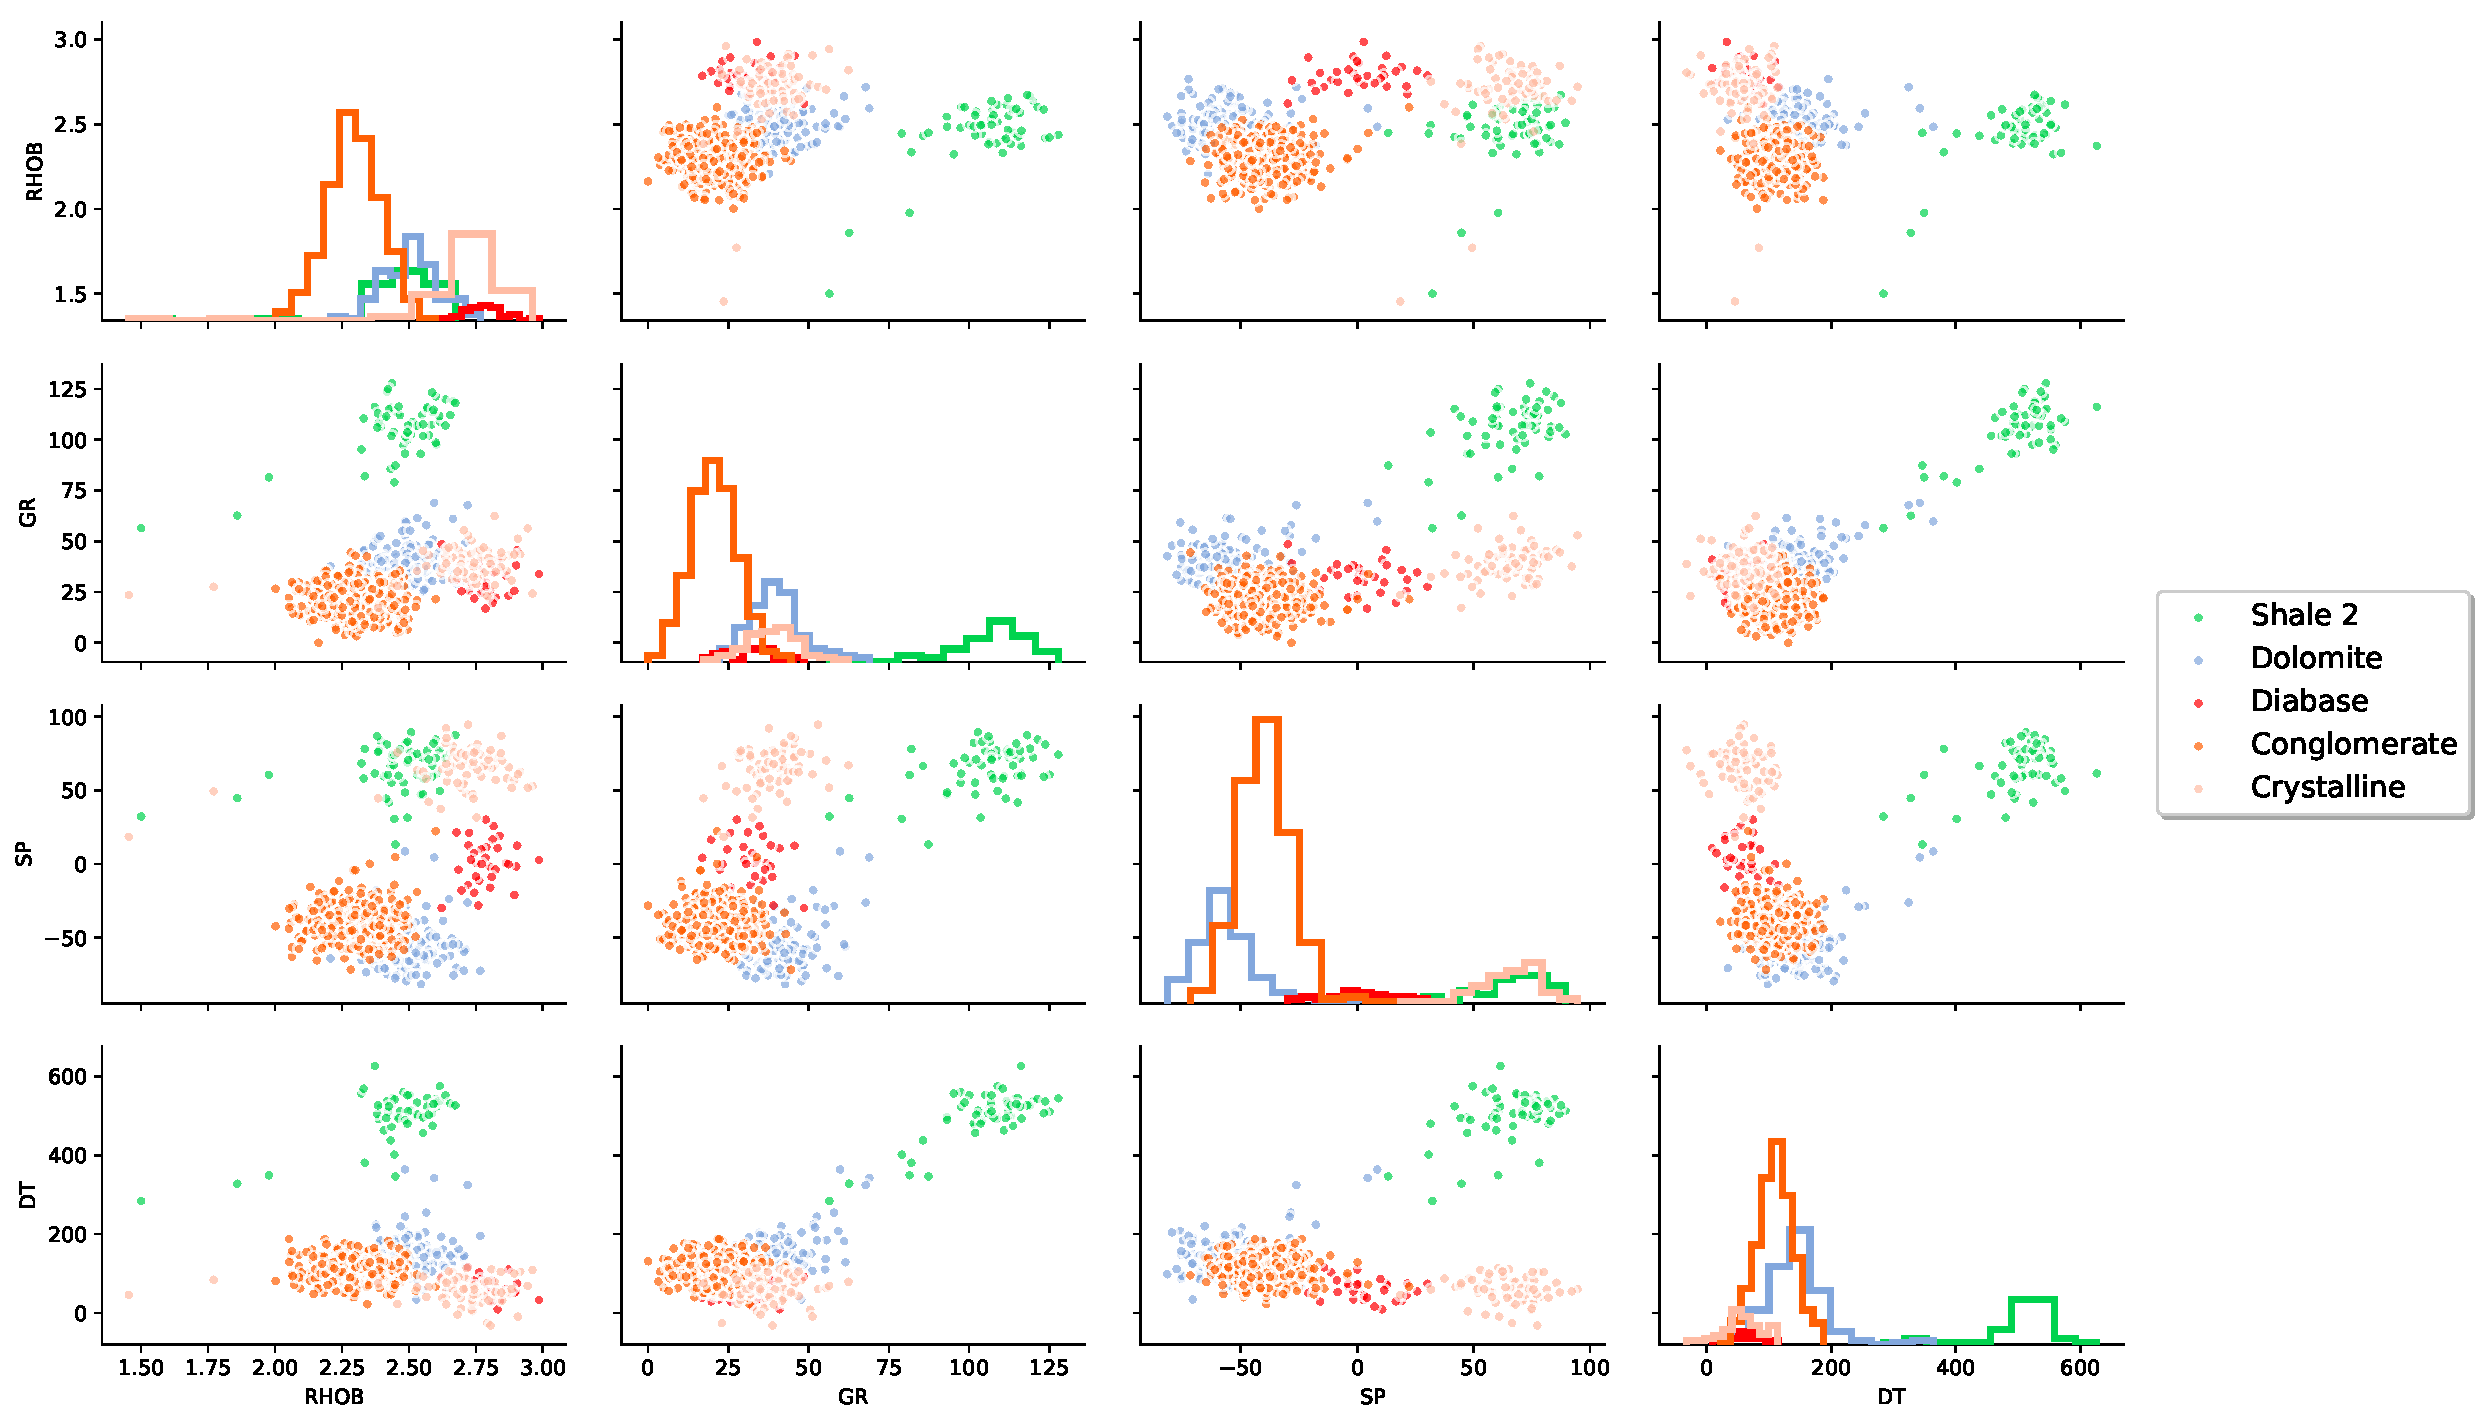
\includegraphics[scale=0.40]{imagens/C1dispersion_convolved.pdf}
	\caption{Dispersion analysis for $C1$ log data. }
	\label{fig:C1_disp}
\end{figure}





\subsection{Classification well C2}

In this second synthetic test, we intentionally set C2 as the classification well. As can be seen in Figure \ref{fig:well_C2} (a), basalt rock unit, located around $3000$ m depth, is missing in the training database. 

. The challenge aspect of this test lies in predicting top-bottom of this unknown rock unit. More generally, we are intended to analyze the capability of each method in working with incomplete training database, which quite common in applications of AI methods in real data cases.  

 Figure \ref{fig:C2_disp} show the dispersion analysis for well C2. As can be seen, 
 
 %(COMENTAR SOBRE AS PRINCIPAIS CARACTERISTICAS OBSERVADAS NOS DADOS E CONFRONTA-LAS COM OS DADOS DE TREINAMENTO, PARA DENUNCIAR ALGUM PADRAO INTERESSANTE ENTRE OS DADOS DE CLASSIFICACAO E O DE TREINAMENTO). 
\begin{figure*}[!htb]
	\centering
	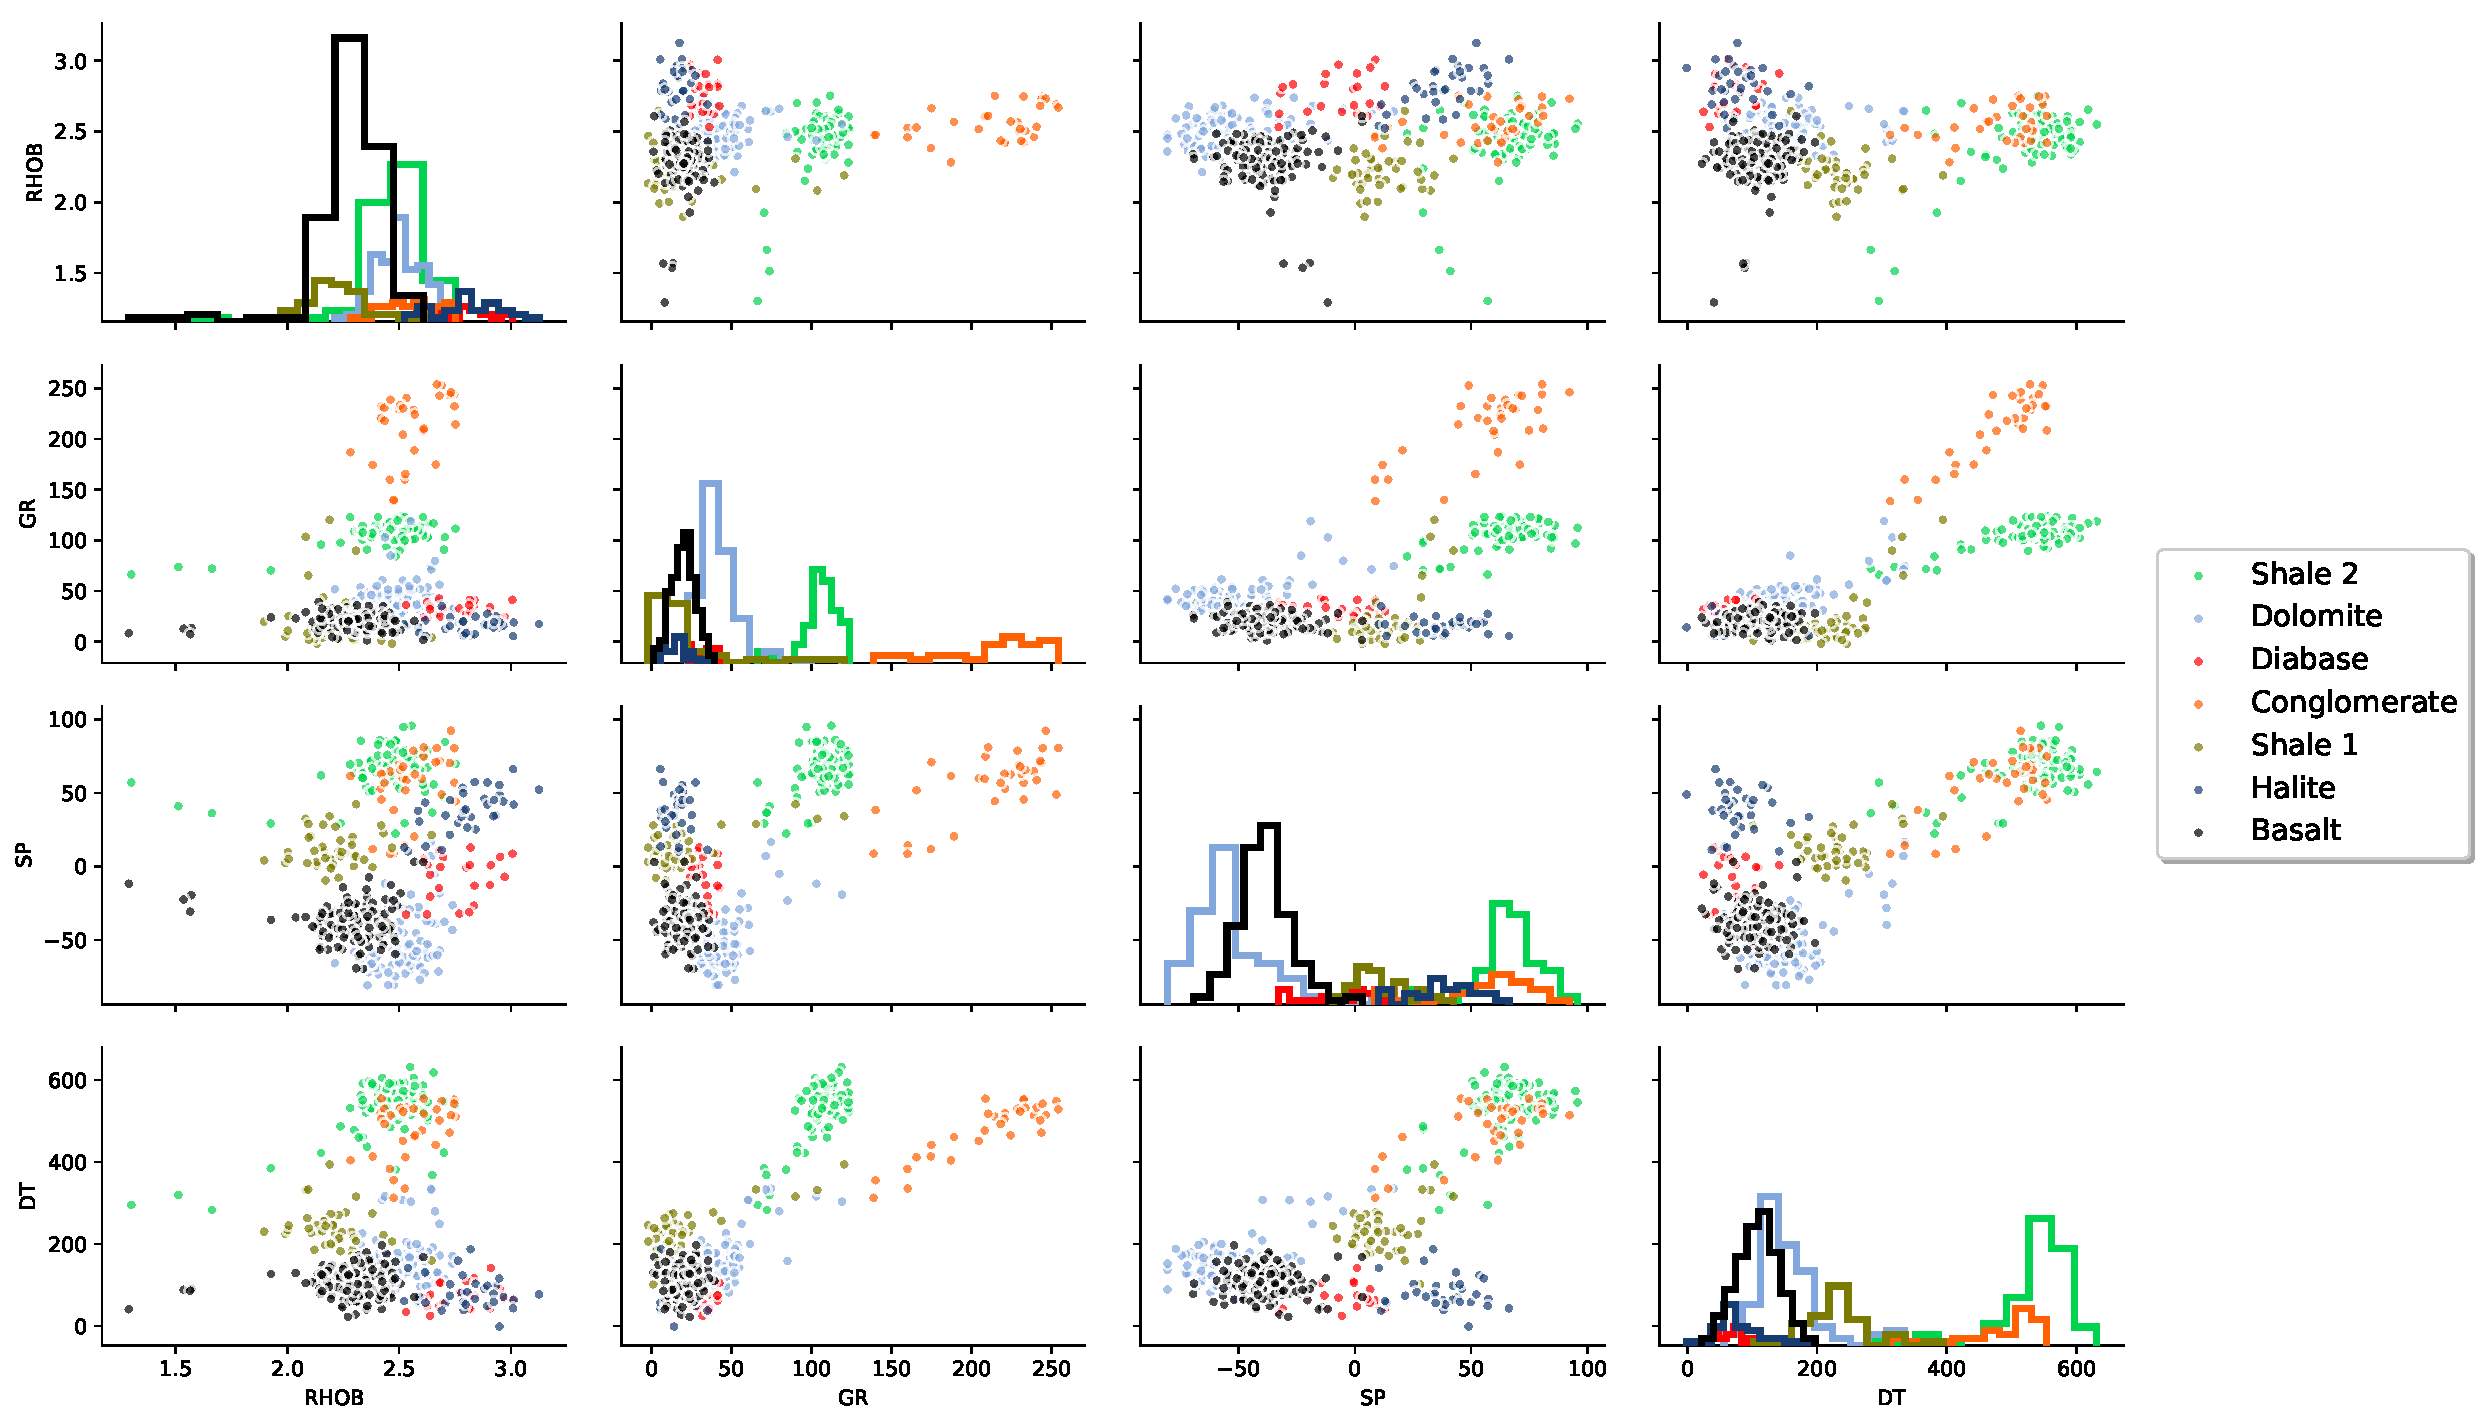
\includegraphics[scale=0.40]{imagens/C2dispersion_convolvido.pdf}
	\caption{Dispersion analysis for $C2$ log data. }
	\label{fig:C2_disp}
\end{figure*}




\subsection{Classification well C3}
\begin{figure*}[!htb]
	\centering
	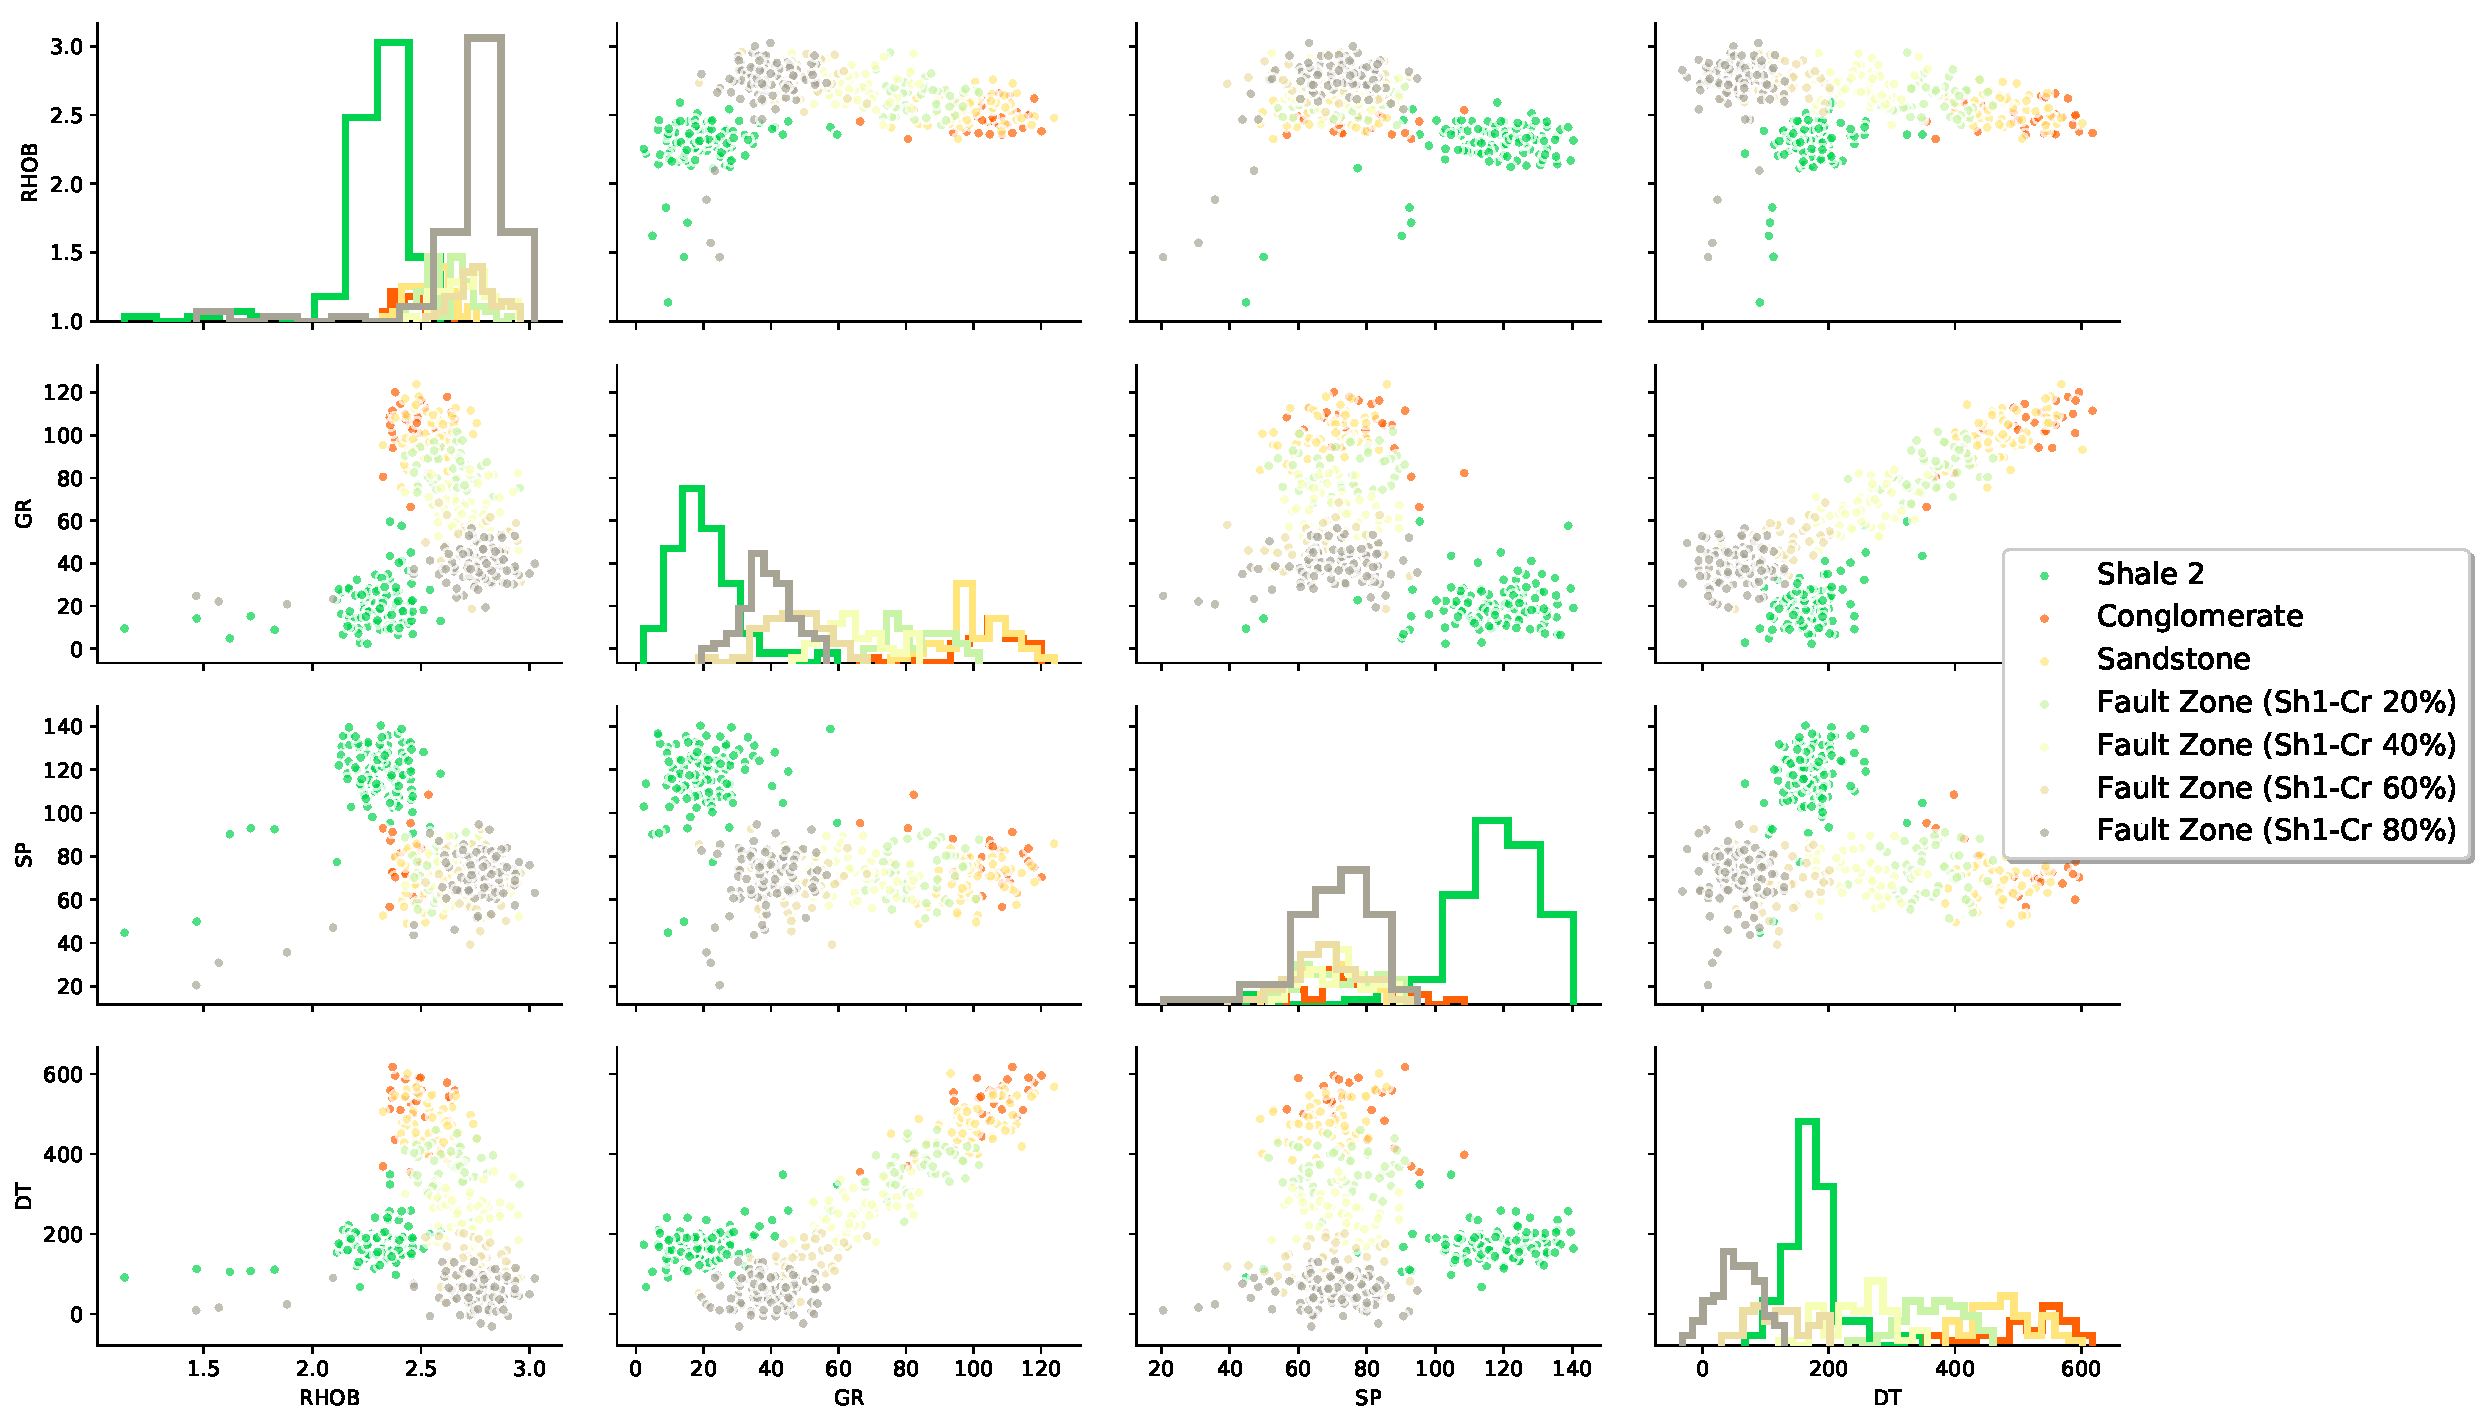
\includegraphics[scale=0.38]{imagens/C3dispersion_convolvido.pdf}
	\caption{ Dispersion analysis for $C3$ log data.  }
	\label{fig:C3_disp}
\end{figure*}




\section{Results with synthetic log data}
\label{sec:Res}
To inspect the capability of each method presented in section \ref{sec:MetAp} to identify rock units, we first design controlled tests comprising wells of the synthetic sedimentary basin presented in section \ref{sec:SynGeo}. All rock units are known, as shown in the Lithological log of Figure \ref{fig:Model}. After that, we apply the same methodology to the real log data of Parana sedimentary basin, in South Brazil (see Figure \ref{fig:Geomap}). 


\subsection{Self-Organizing Map (SOM)}
Figure \ref{fig:SOM} shows the SOM obtained for the training database. We can observe that all rock units are presented in the cortex map, as can be seen in Figure \ref{fig:SOM}a. Additionally, the convergence curve of Figure \ref{fig:SOM}b reinforces the good training process for the synthetic examples. We set the cortex with $400$ neurons ($20$ $\times$ $20$) and $3000$ iterations for computing the weights. 
\begin{figure*}[ht!]
	\begin{center}
		\subfloat[][]
		{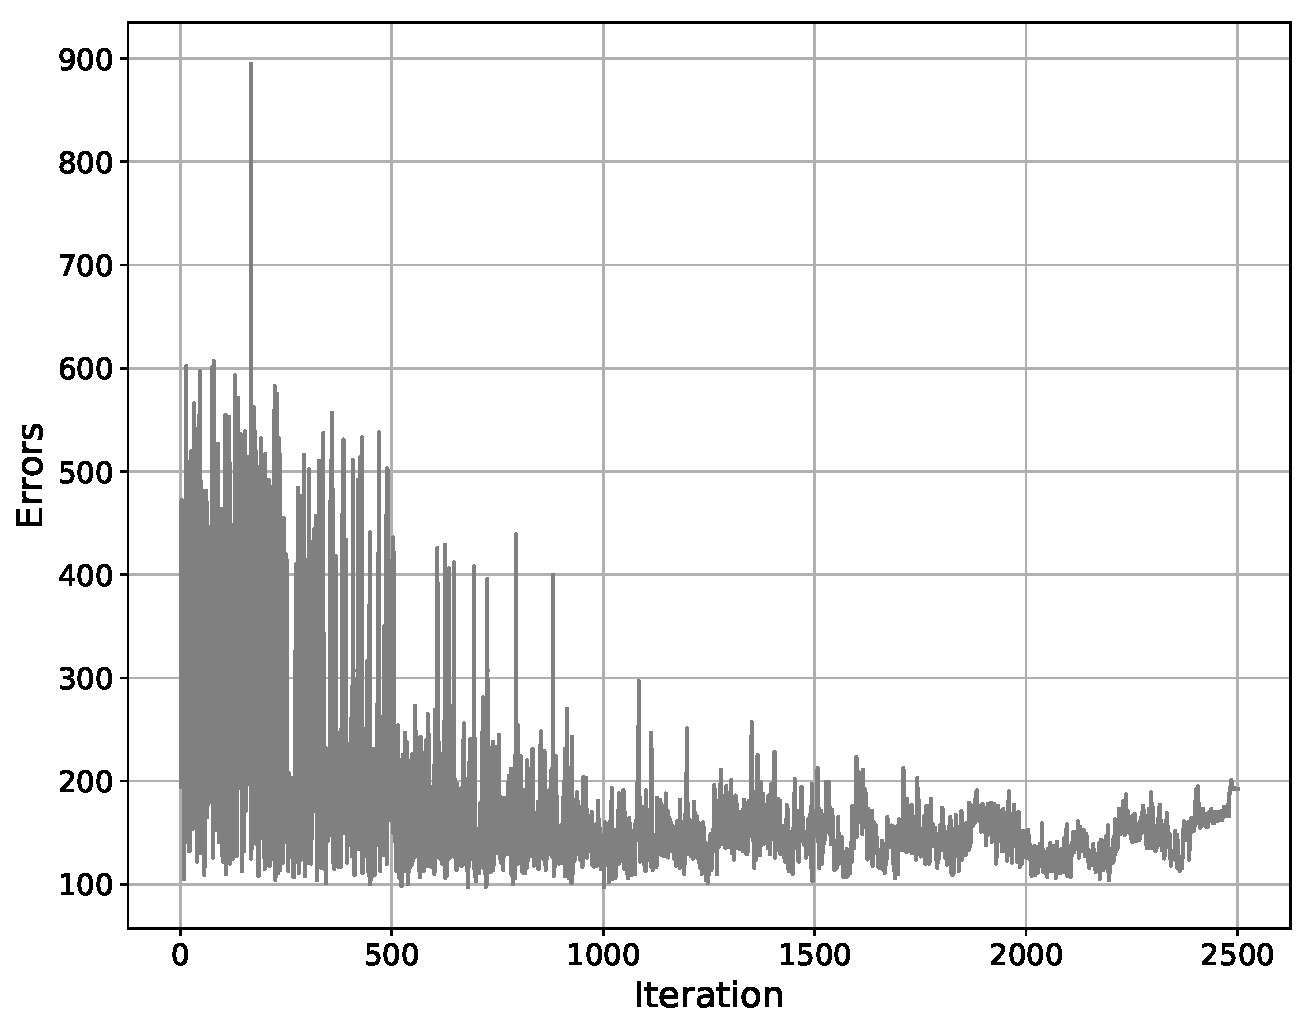
\includegraphics[scale=0.30]{imagens/Conv_sint.pdf}}
		\subfloat[]
		{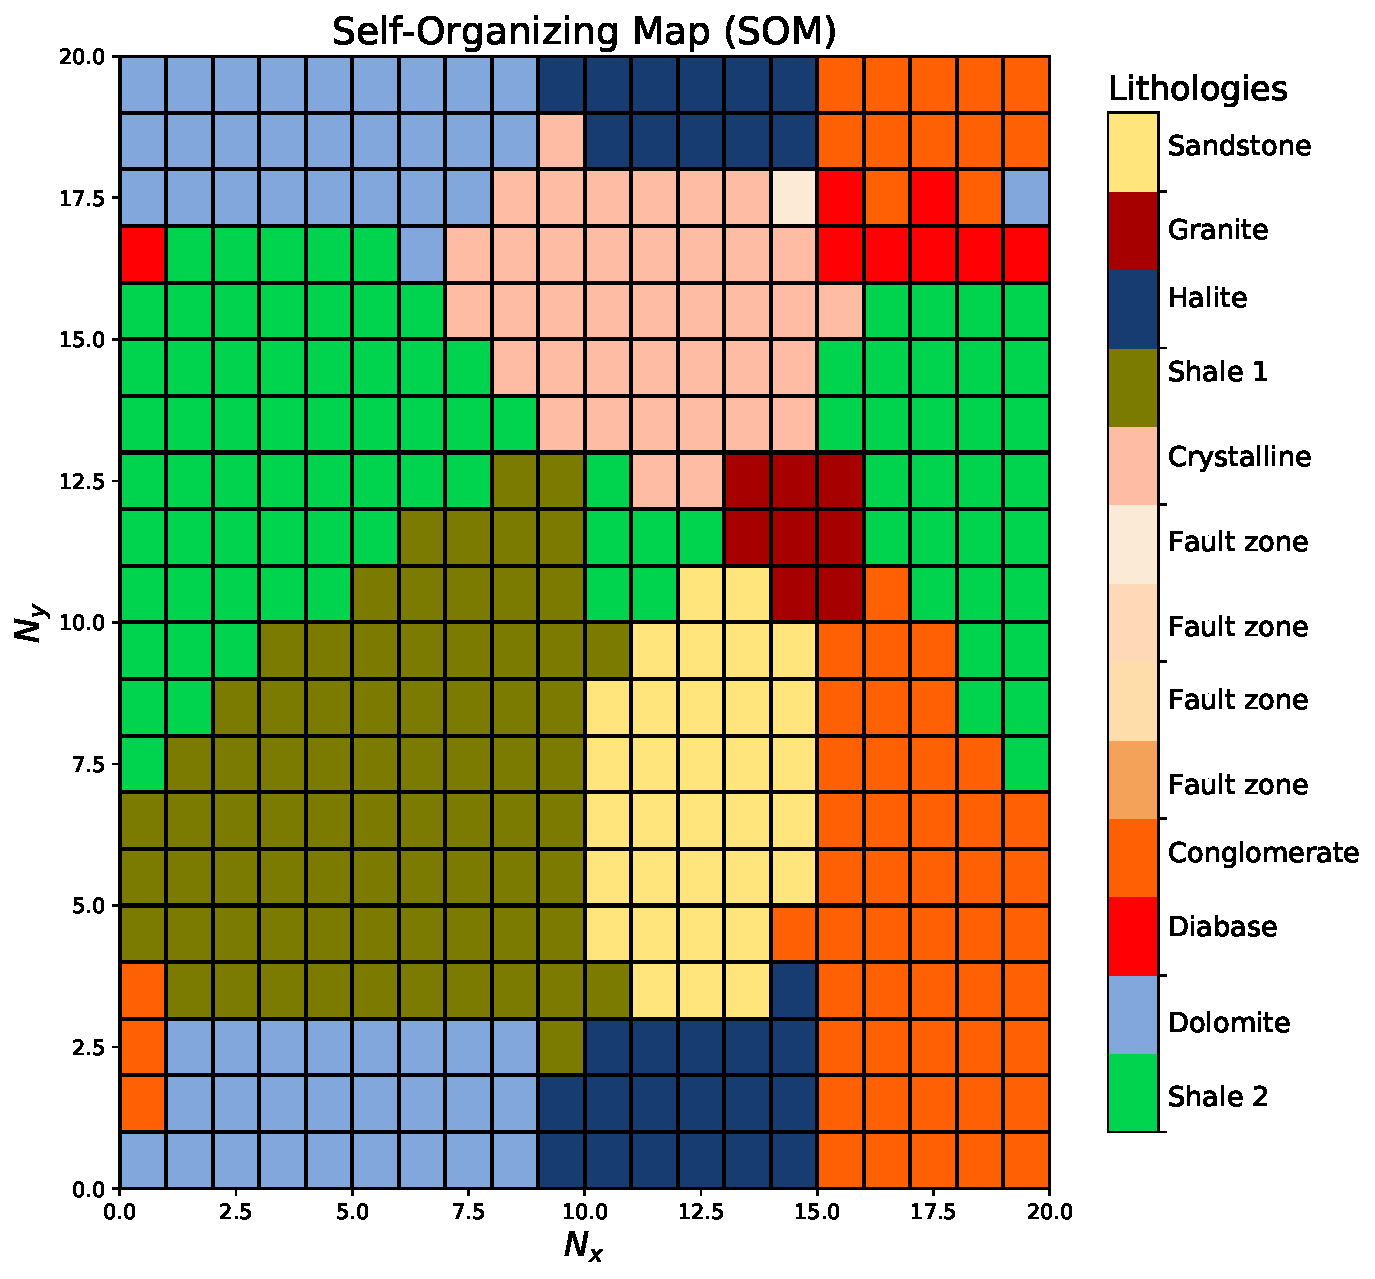
\includegraphics[scale=0.30]{imagens/cortex.pdf}}
		\caption{ (a) Convergence analysis for the SOM training stage. (b) SOM for the synthetic training database. Colors highlight each lithology identified in the cortex.}
		\label{fig:SOM}
	\end{center}
\end{figure*}
Each training well presents a specific geological configuration to produce a consistent training database. The classification wells are detailed in subsections \ref{subsub:C1}, \ref{subsub:C2} and \ref{subsub:C3}.

\subsection{WELL C1}
\label{subsub:C1}
\begin{figure}[!htb]
	\centering
	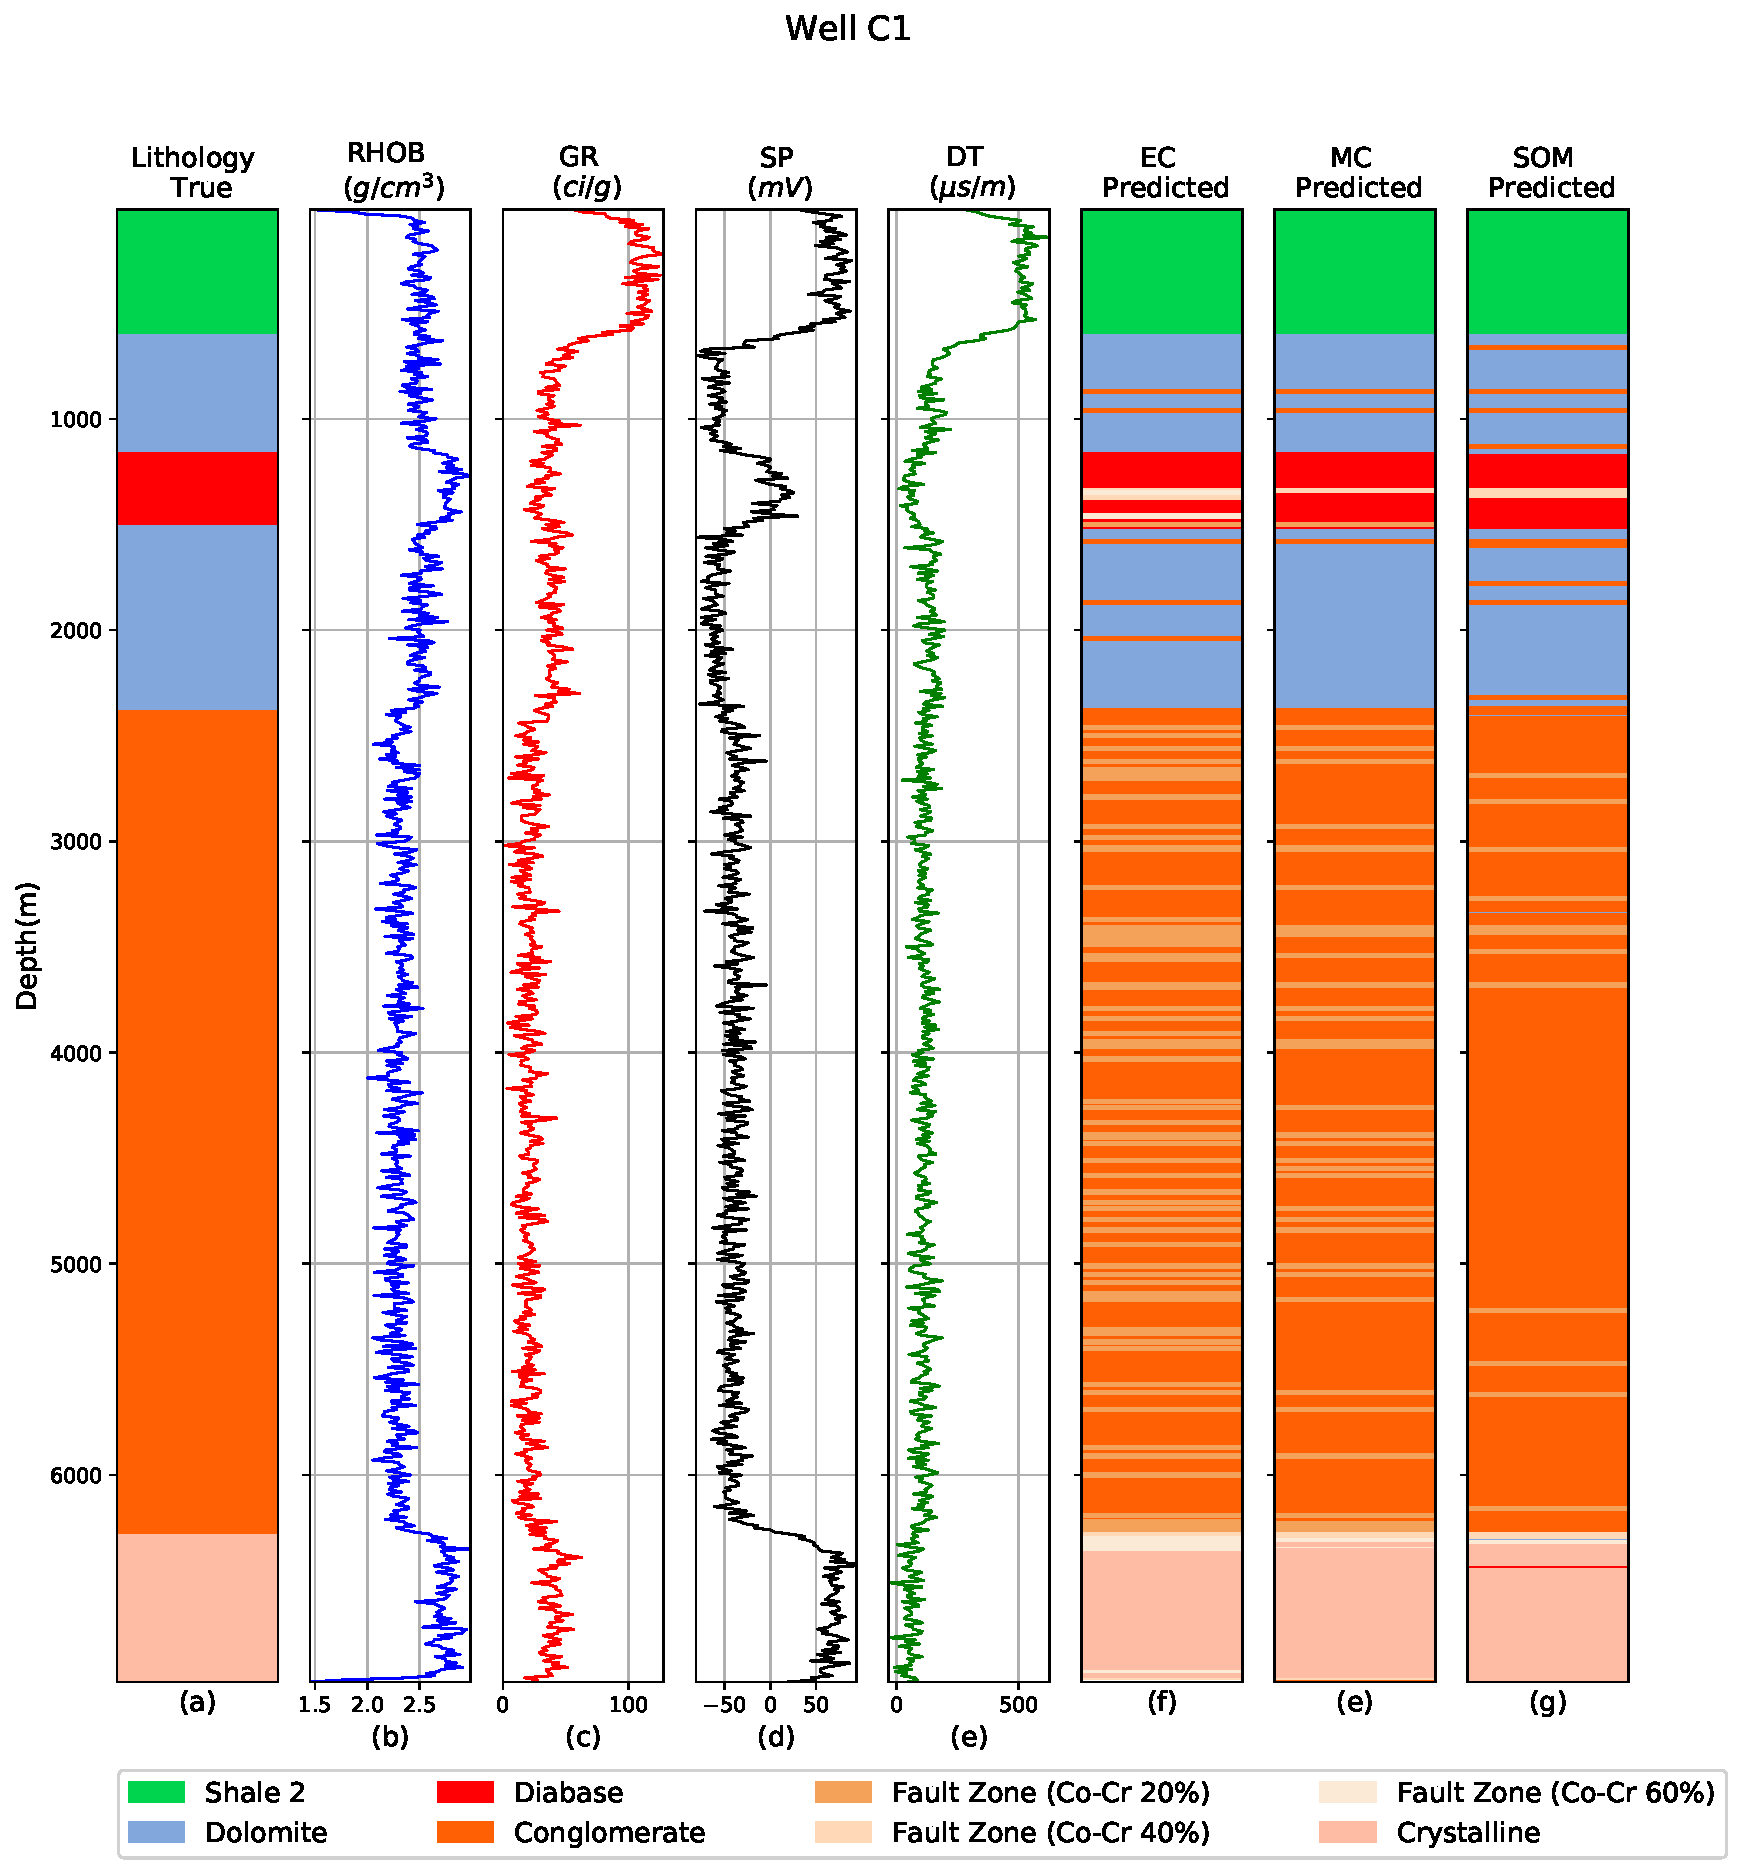
\includegraphics[scale=0.55]{imagens/wellC1nx80v02.pdf}
	\caption{Results for synthetic well C1.  }
	\label{fig:well_C1}
\end{figure}

\begin{figure*}[ht!]
	\begin{center}
		\subfloat[][]
		{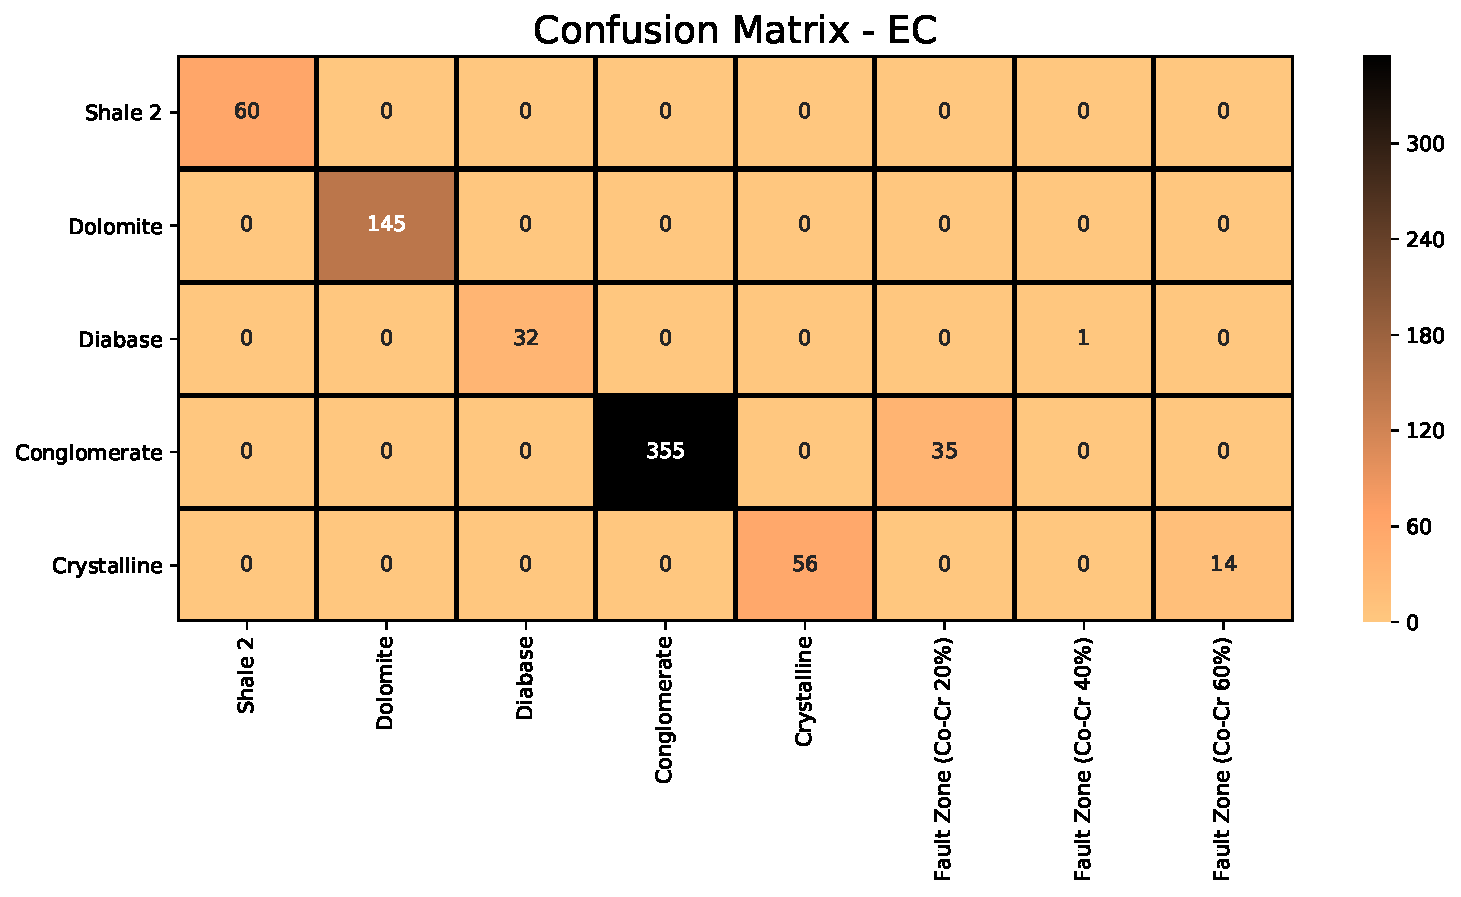
\includegraphics[scale=0.32]{imagens/CM_Eucli_C1.pdf}}
		\subfloat[]
		{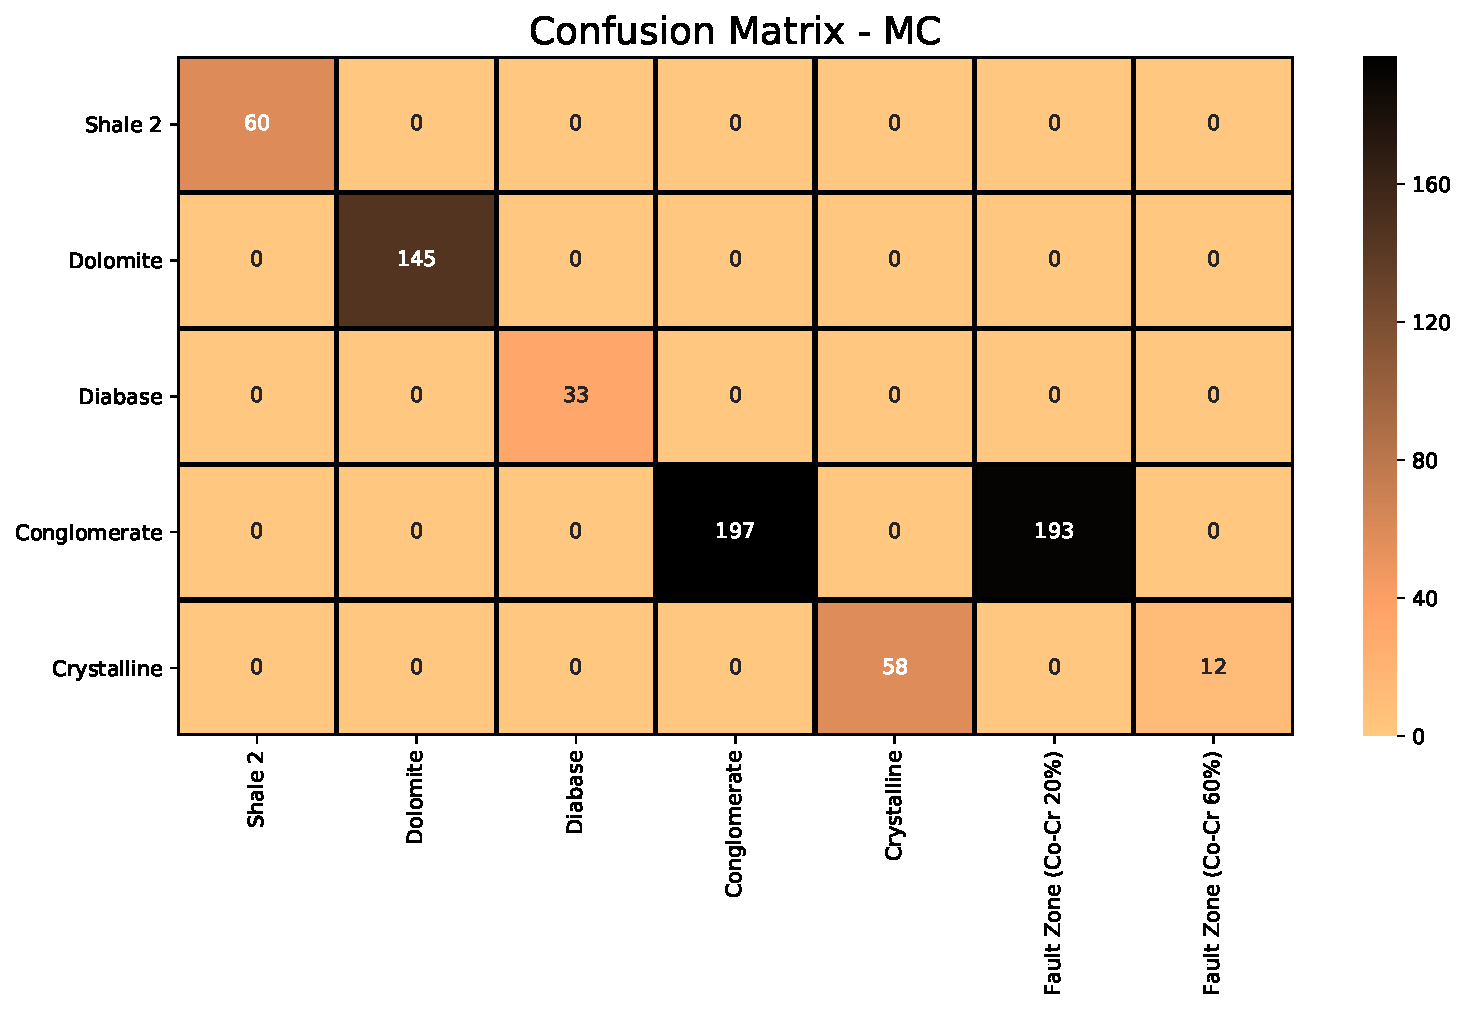
\includegraphics[scale=0.32]{imagens/CM_Maha_C1.pdf}} \\
		\subfloat[]
		{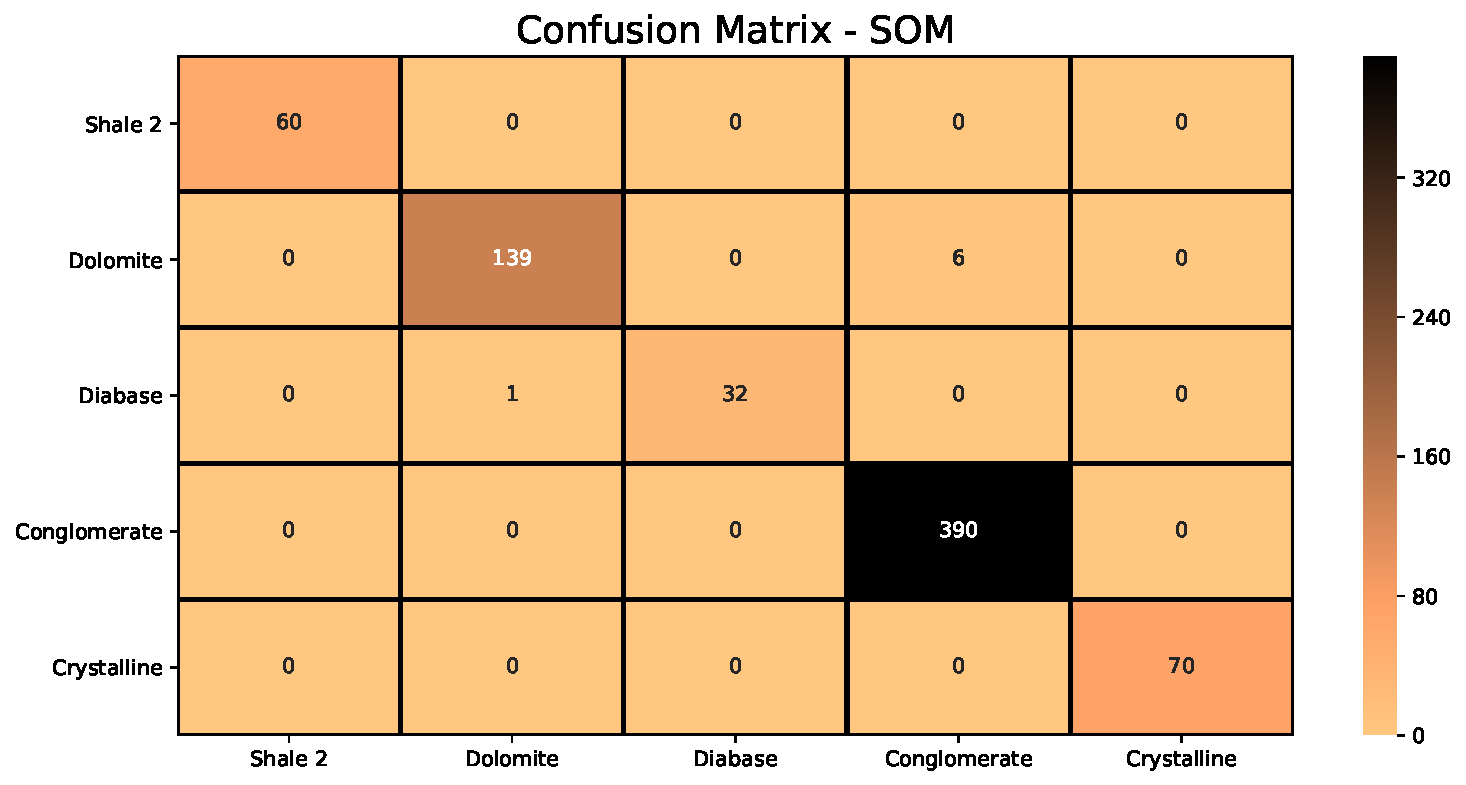
\includegraphics[scale=0.32]{imagens/CM_Kohonen_C1.pdf}} 
		\caption{ Confusion Matrix for (a) Euclidean Classifier , (b) Mahalanobis Classifier and (c) Self-Organizing Map}
		\label{fig:CM_C1}
	\end{center}
\end{figure*}


\subsection{WELL C2}
\label{subsub:C2}
Figure \ref{fig:well_C2} a, b, c, d and e show the true lithological log and the four simulated logs. In this particular example, we can observe some significant "bumps" in the log data comprising diabase, shale 1, halite and basalt rock units. These patterns in the classification data set reinforces the importance of good quality data for accurate prediction of rock units within wells.  
 
\begin{figure}[!htb]
	\centering
	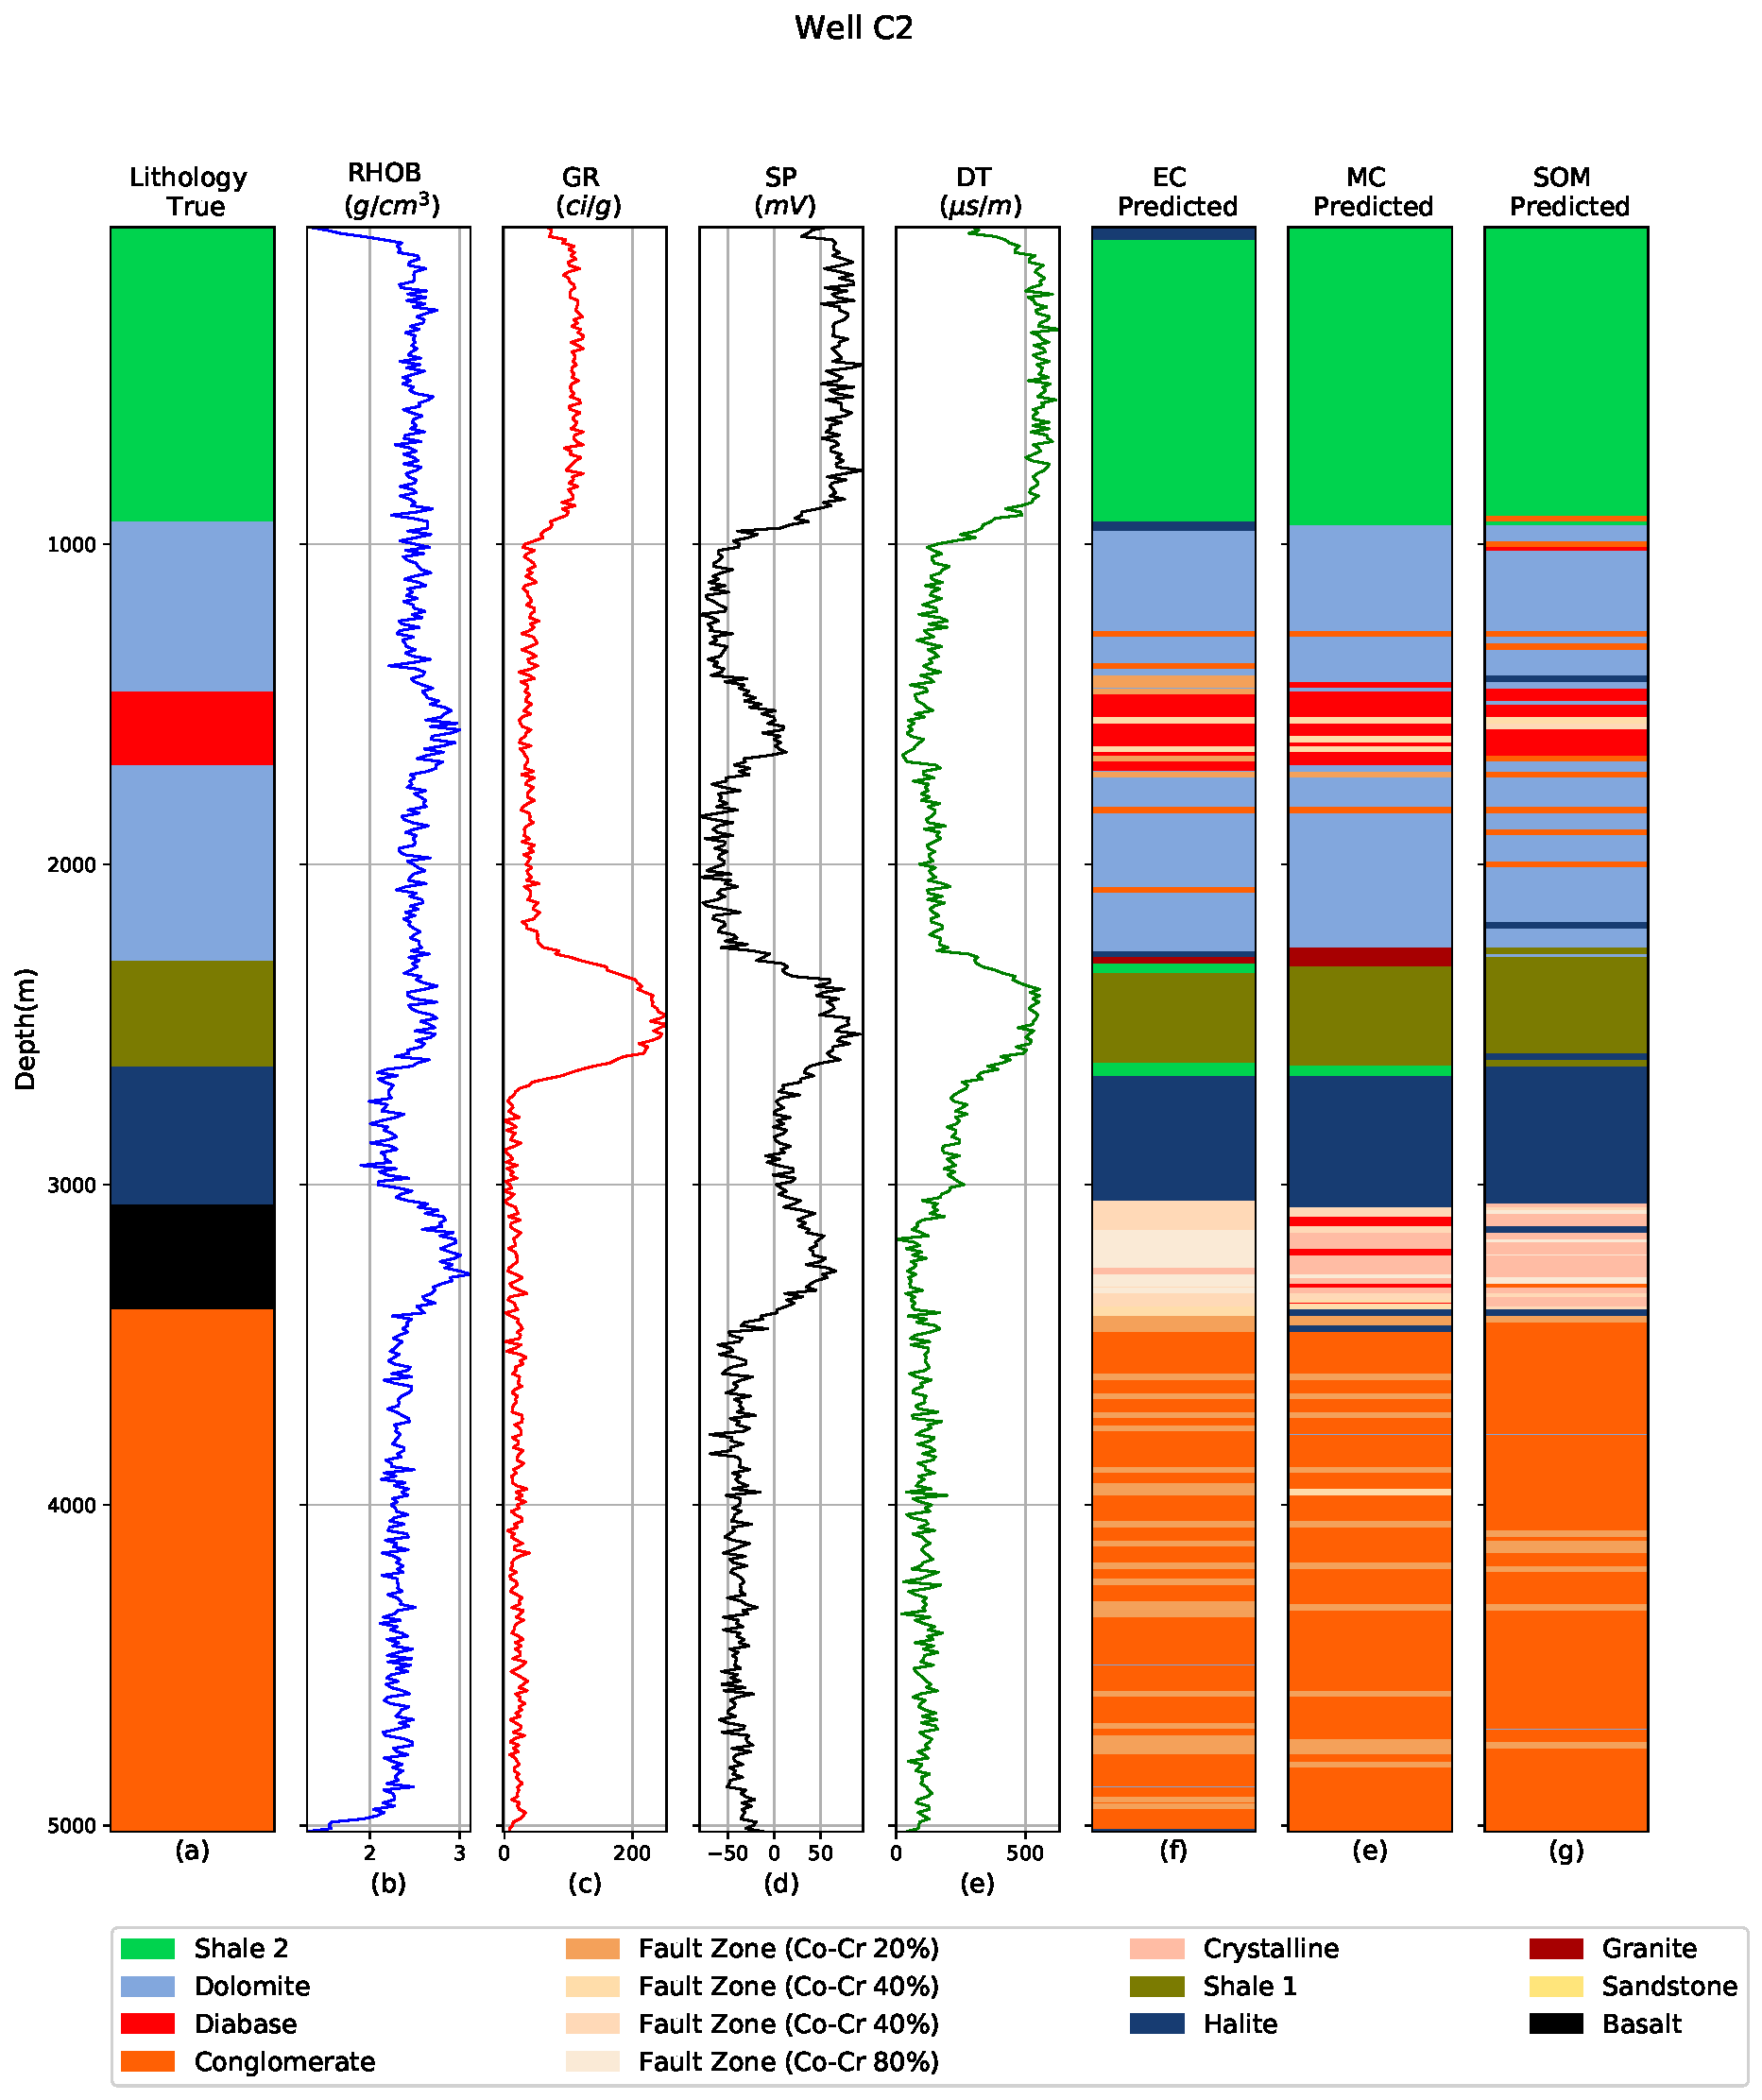
\includegraphics[scale=0.4]{imagens/wellC2nx80v02.pdf}
	\caption{Results for synthetic well C2.  }
	\label{fig:well_C2}
\end{figure}


\begin{figure*}[ht!]
	\begin{center}
		\subfloat[][]
		{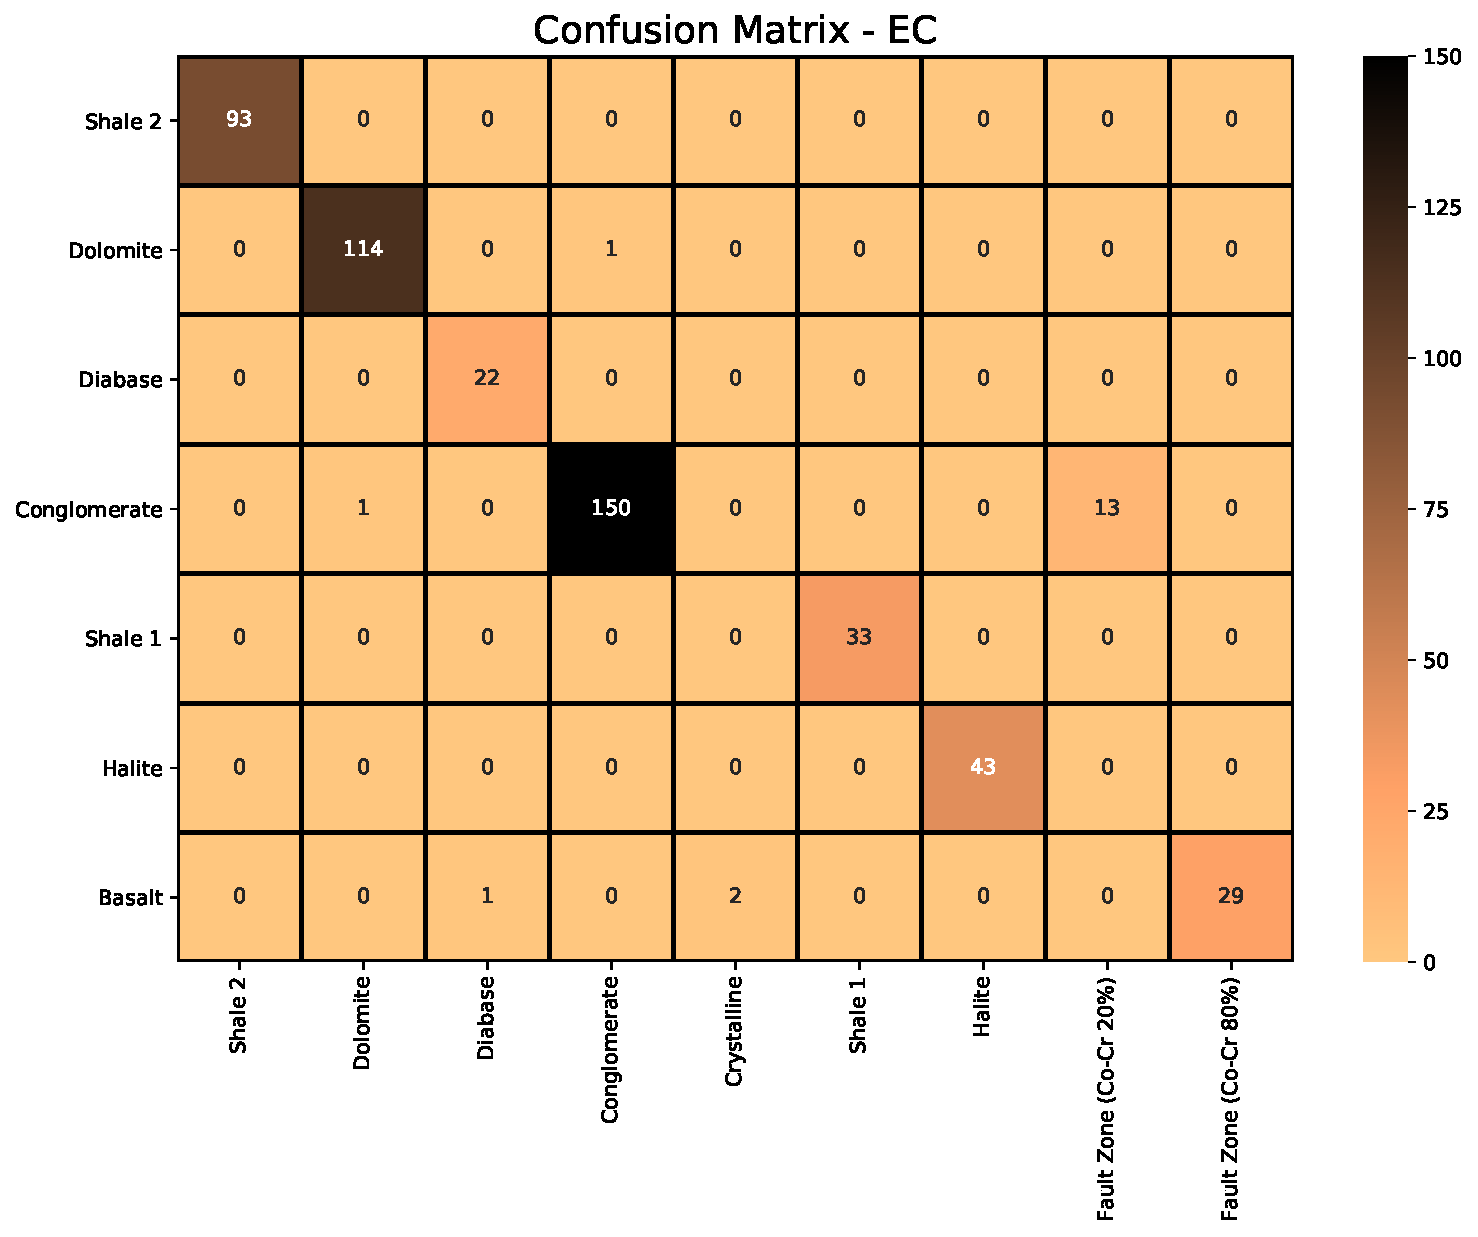
\includegraphics[scale=0.32]{imagens/CM_Eucli_C2.pdf}} 
		\subfloat[]
		{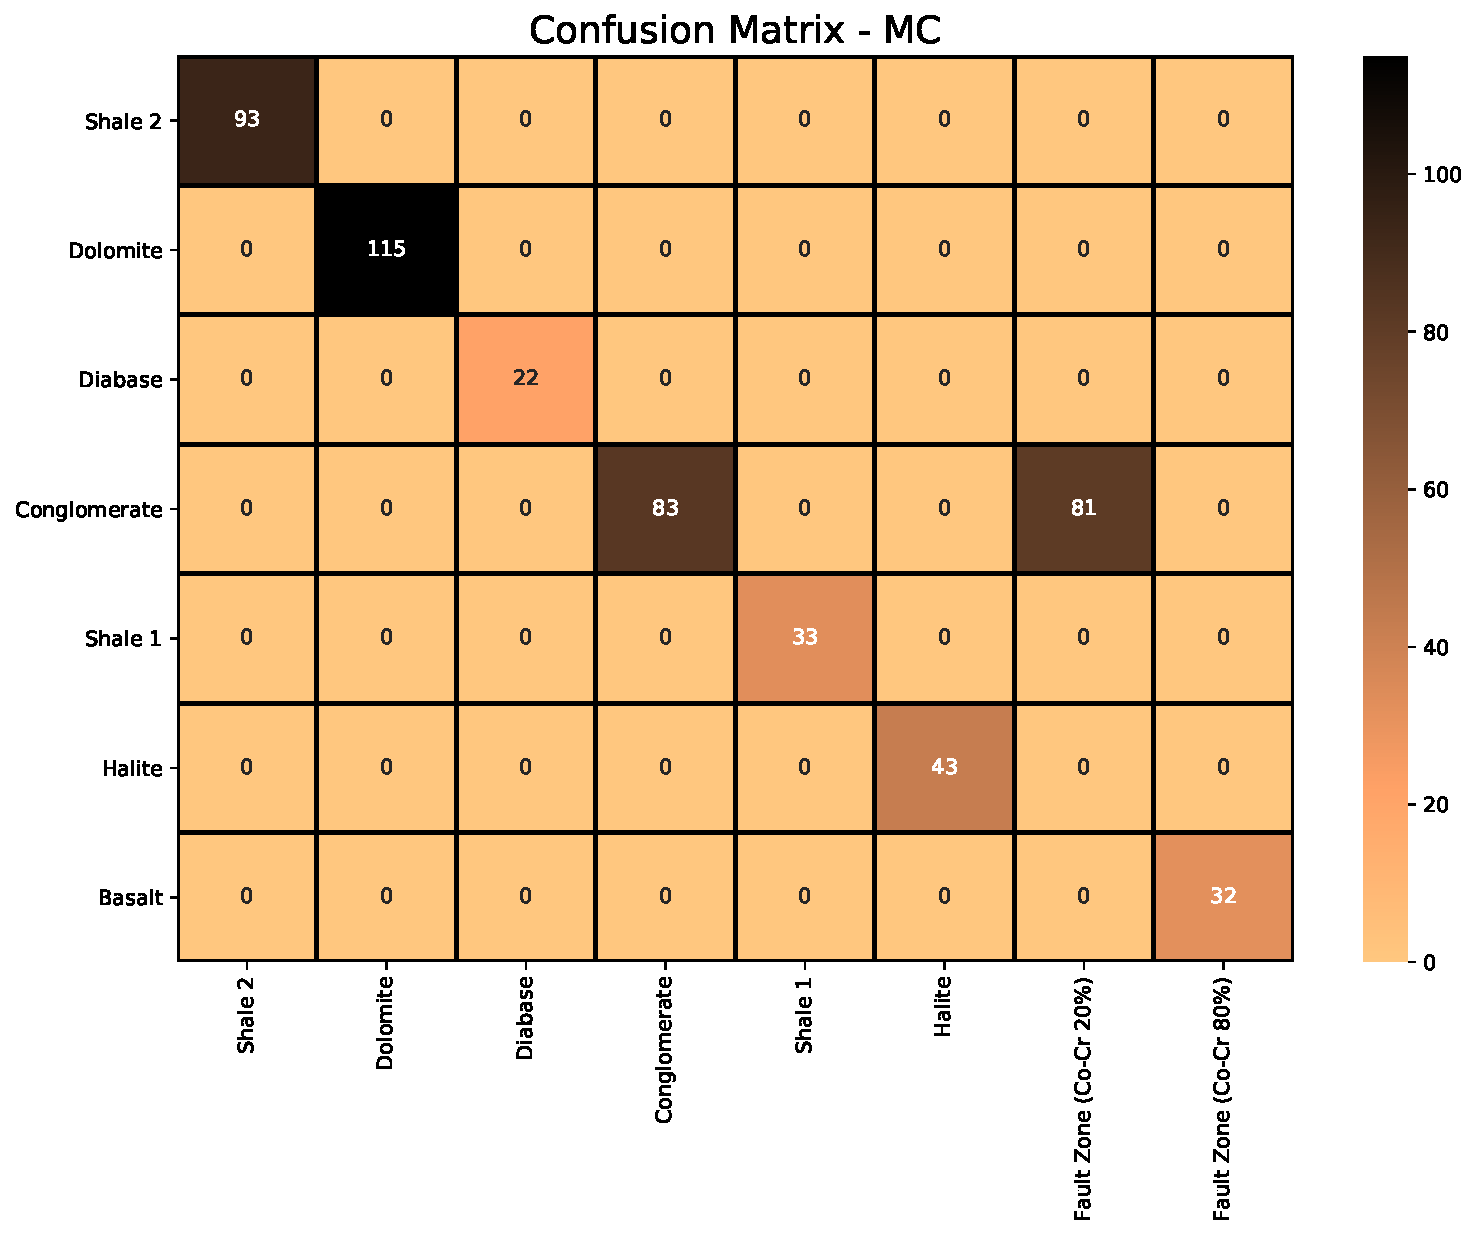
\includegraphics[scale=0.32]{imagens/CM_Maha_C2.pdf}} \\
		\subfloat[]
		{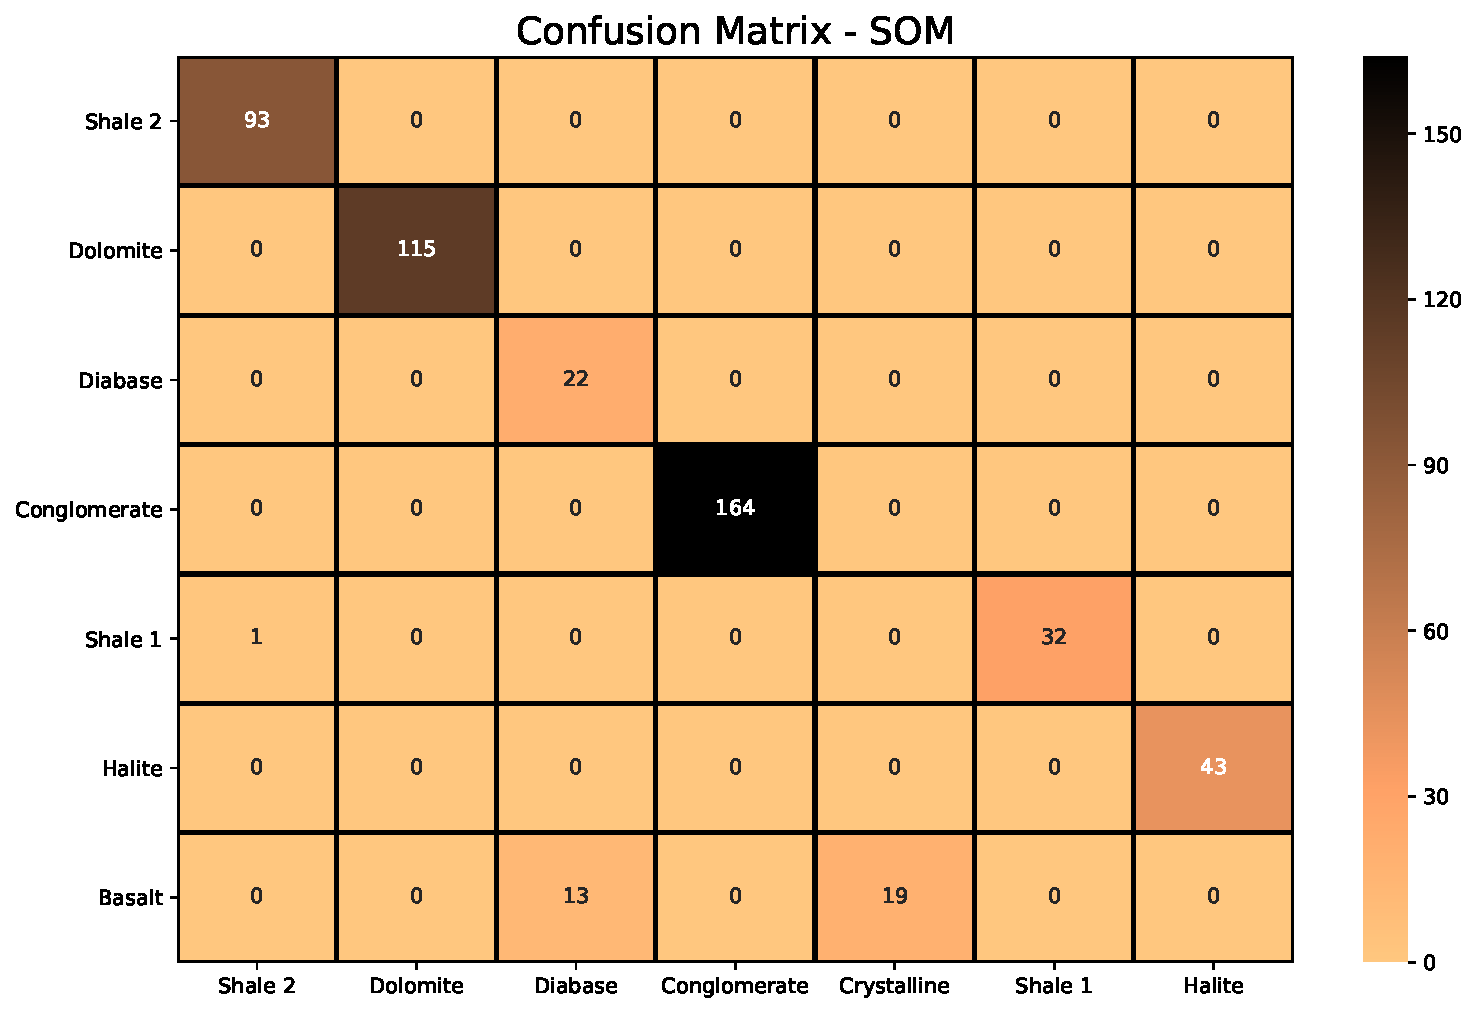
\includegraphics[scale=0.32]{imagens/CM_Kohonen_C2.pdf}} 
		\caption{ Confusion Matrix for (a) Euclidean Classifier , (b) Mahalanobis Classifier and (c) Self-Organizing Map}
		\label{fig:CM_C2}
	\end{center}
\end{figure*}

\subsection{WELL C3}
\label{subsub:C3}


\begin{figure}[!htb]
	\centering
	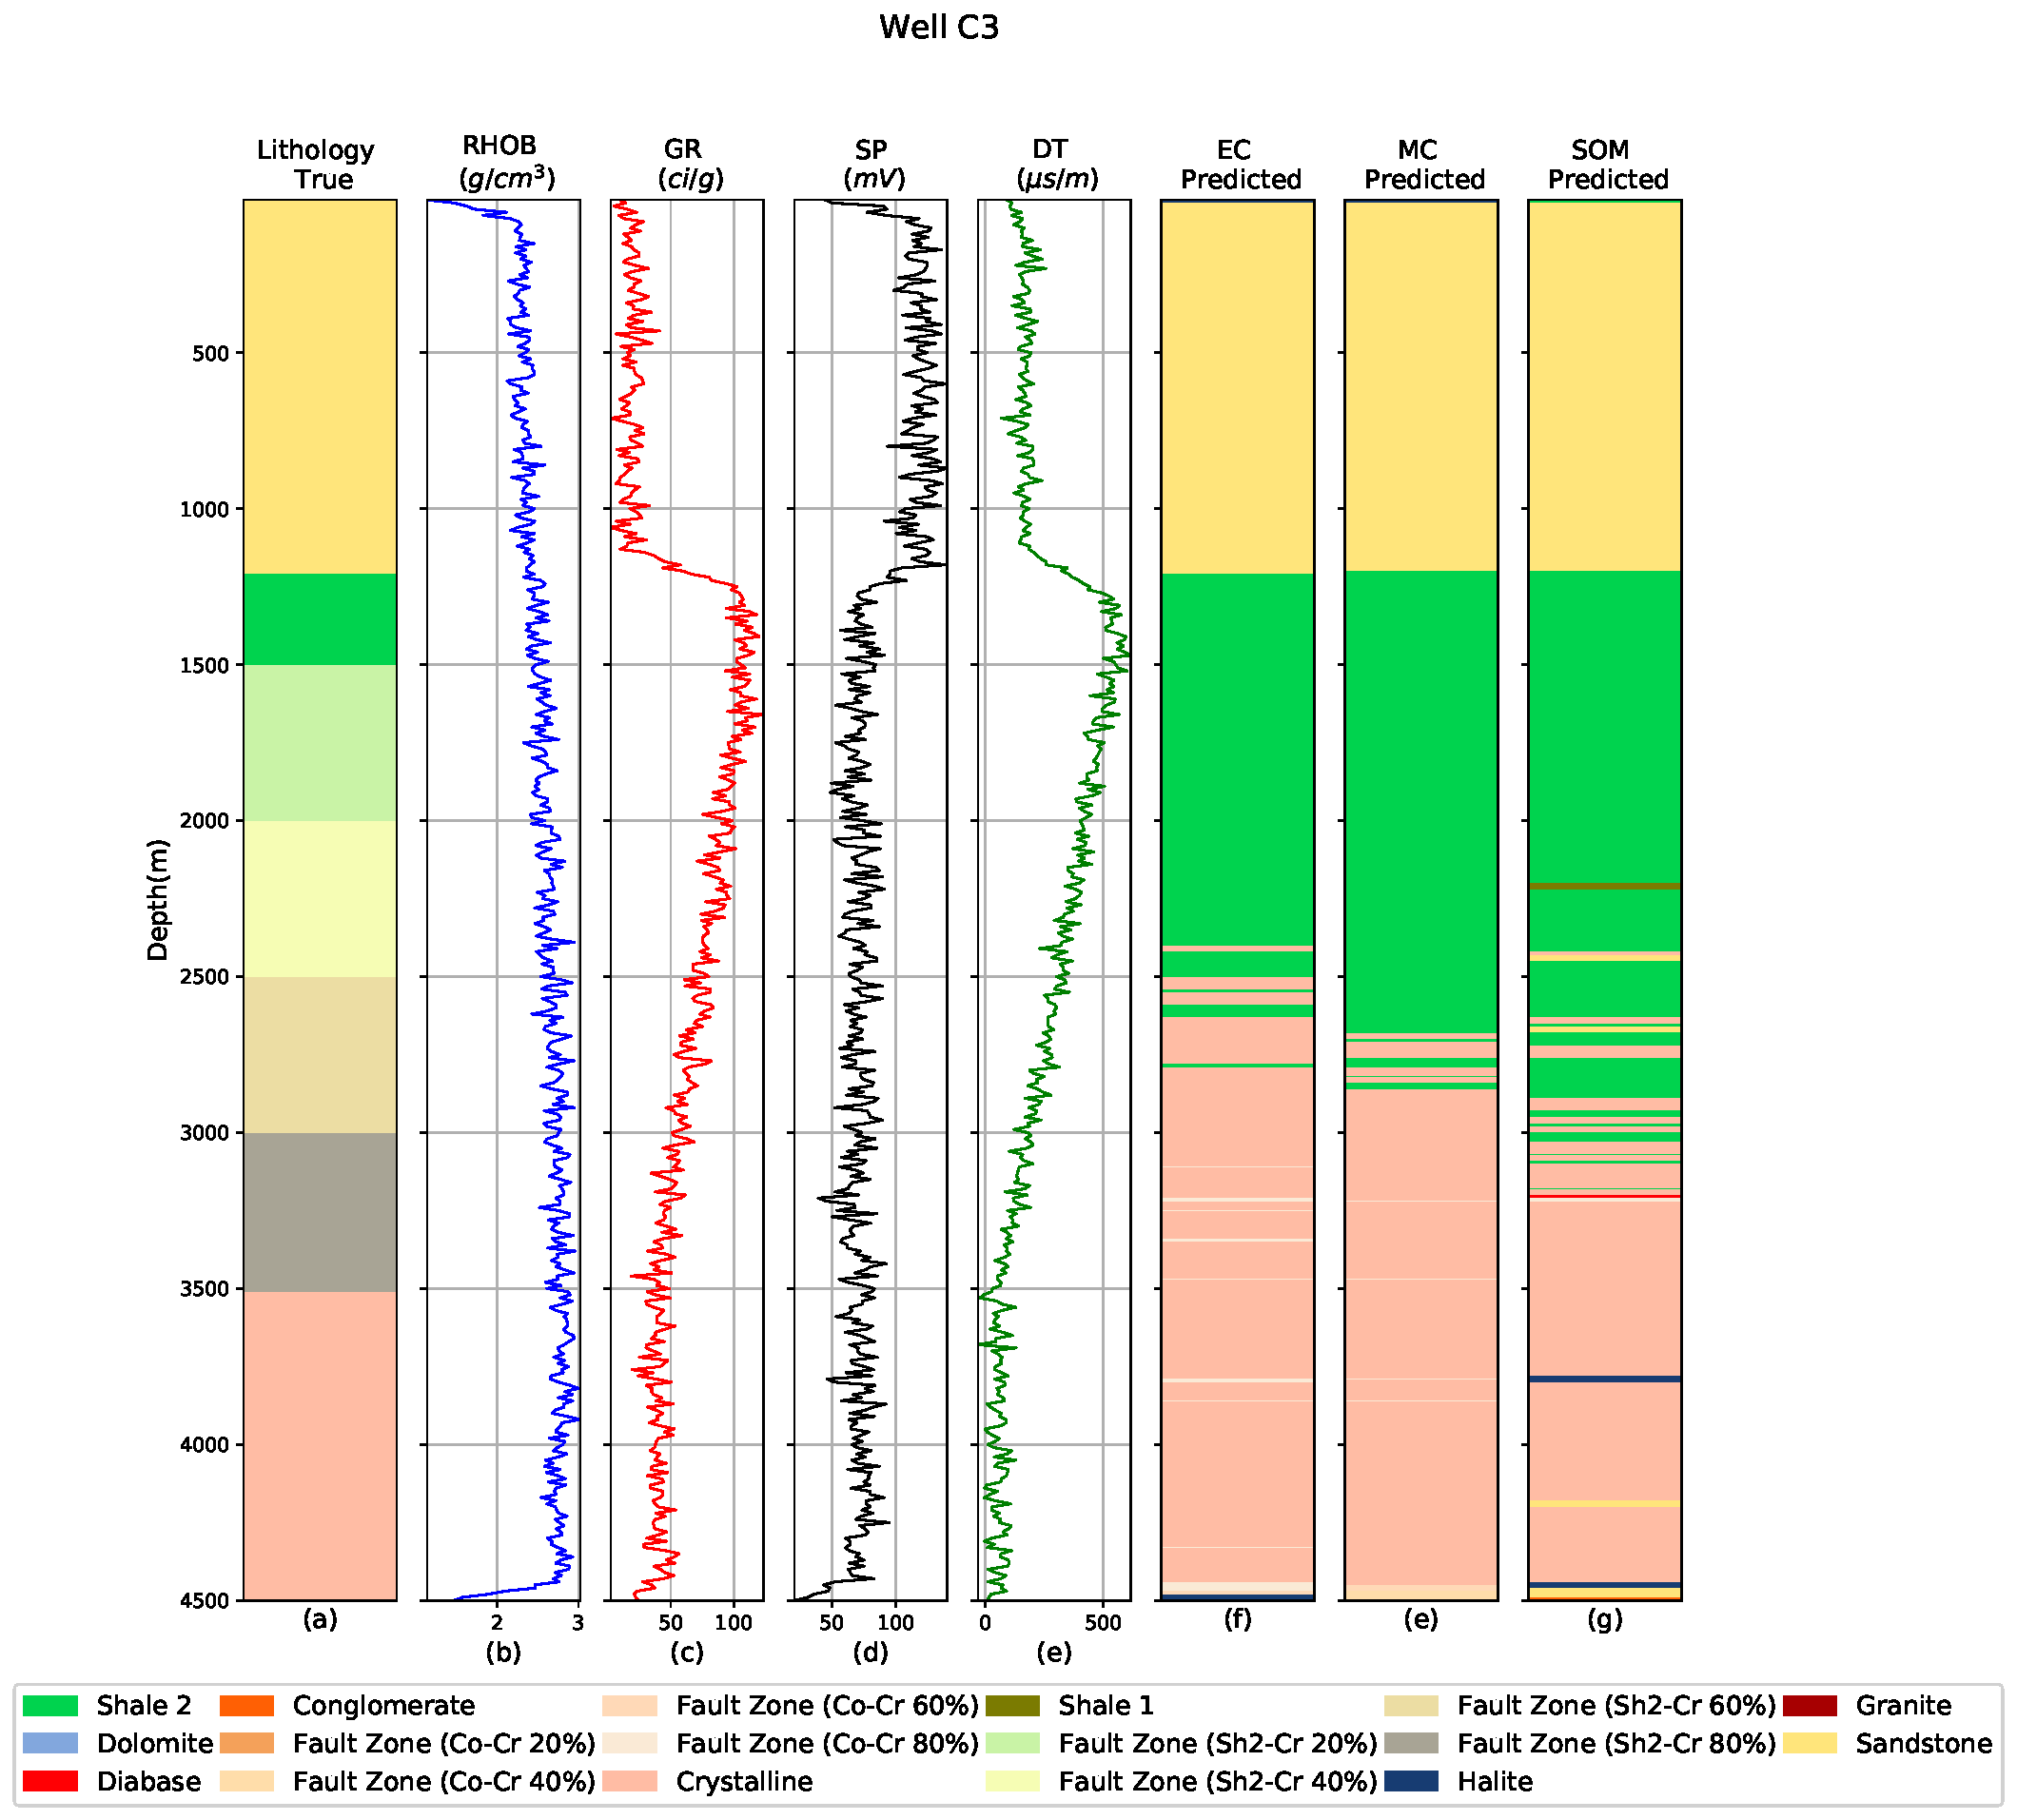
\includegraphics[scale=0.4]{imagens/wellC3nx80v02.pdf}
	\caption{Results for synthetic well C3.  }
	\label{fig:well_C3}
\end{figure}

\begin{figure*}[ht!]
	\begin{center}
		\subfloat[][]
		{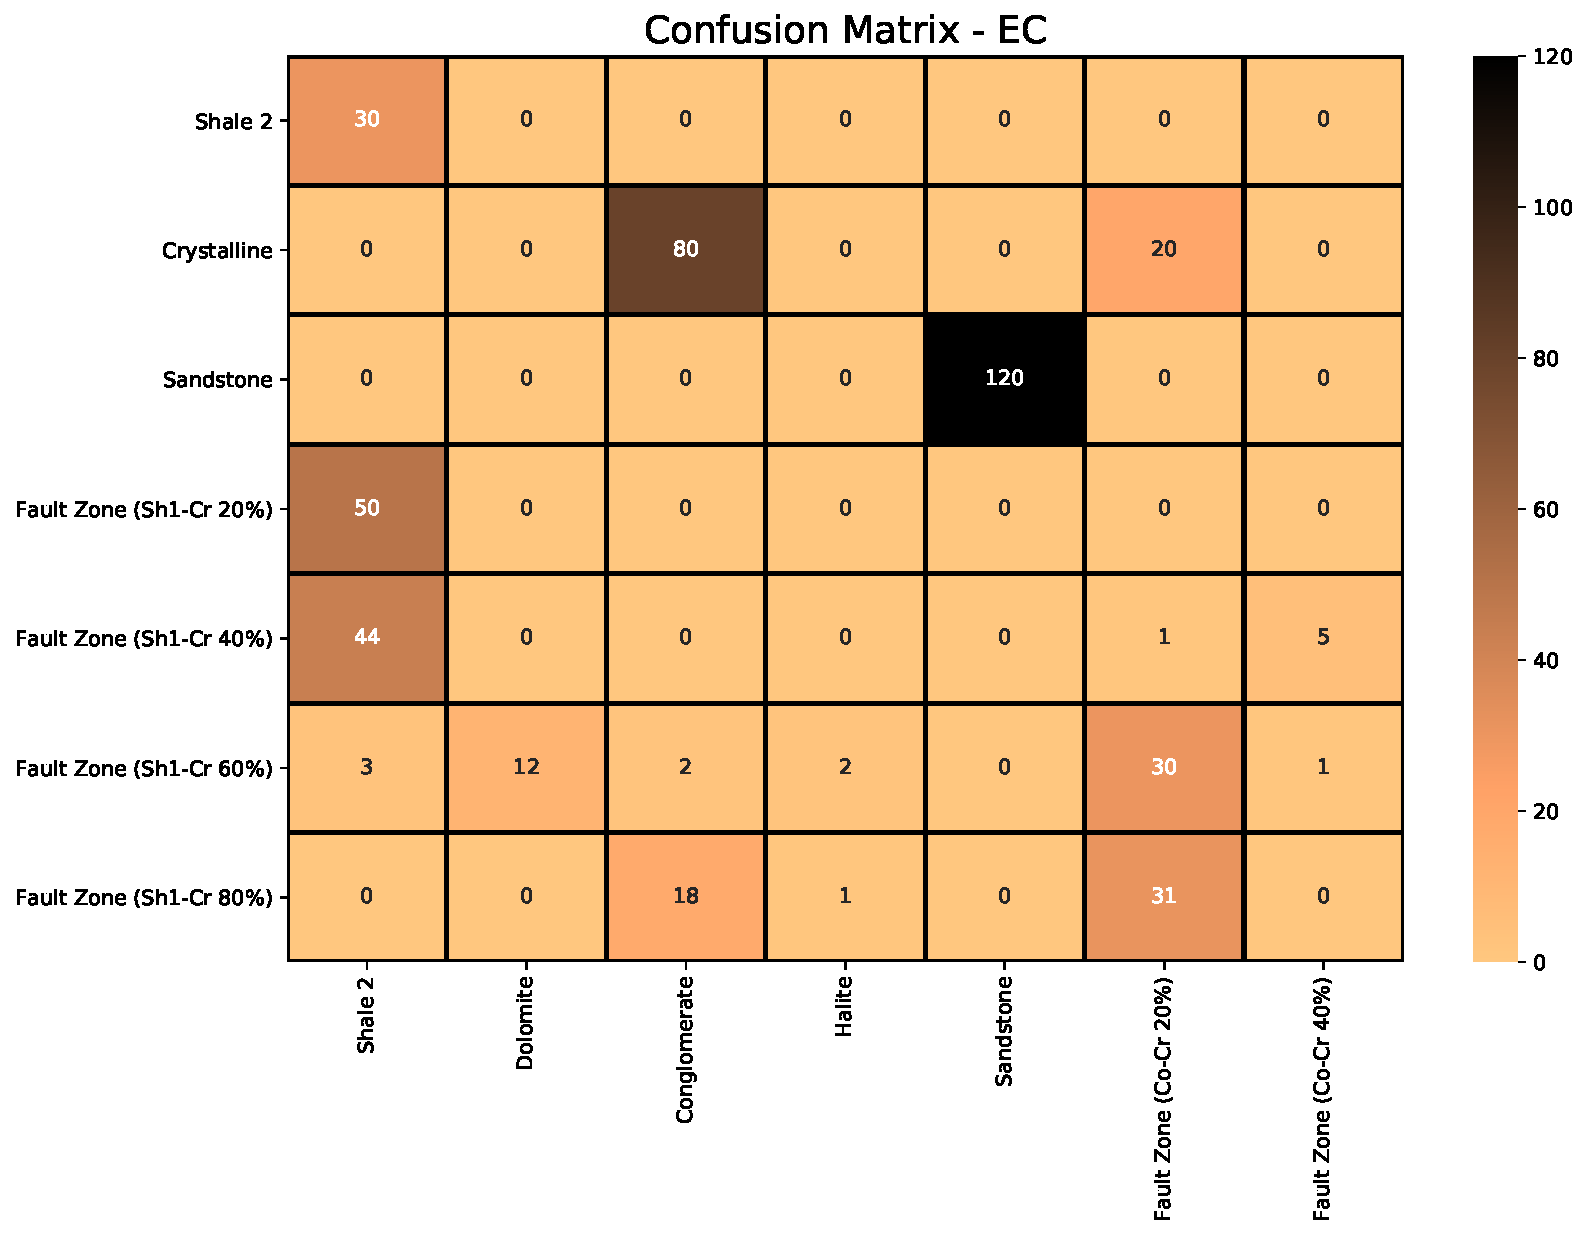
\includegraphics[scale=0.32]{imagens/CM_Eucli_C3.pdf}} 
		\subfloat[]
		{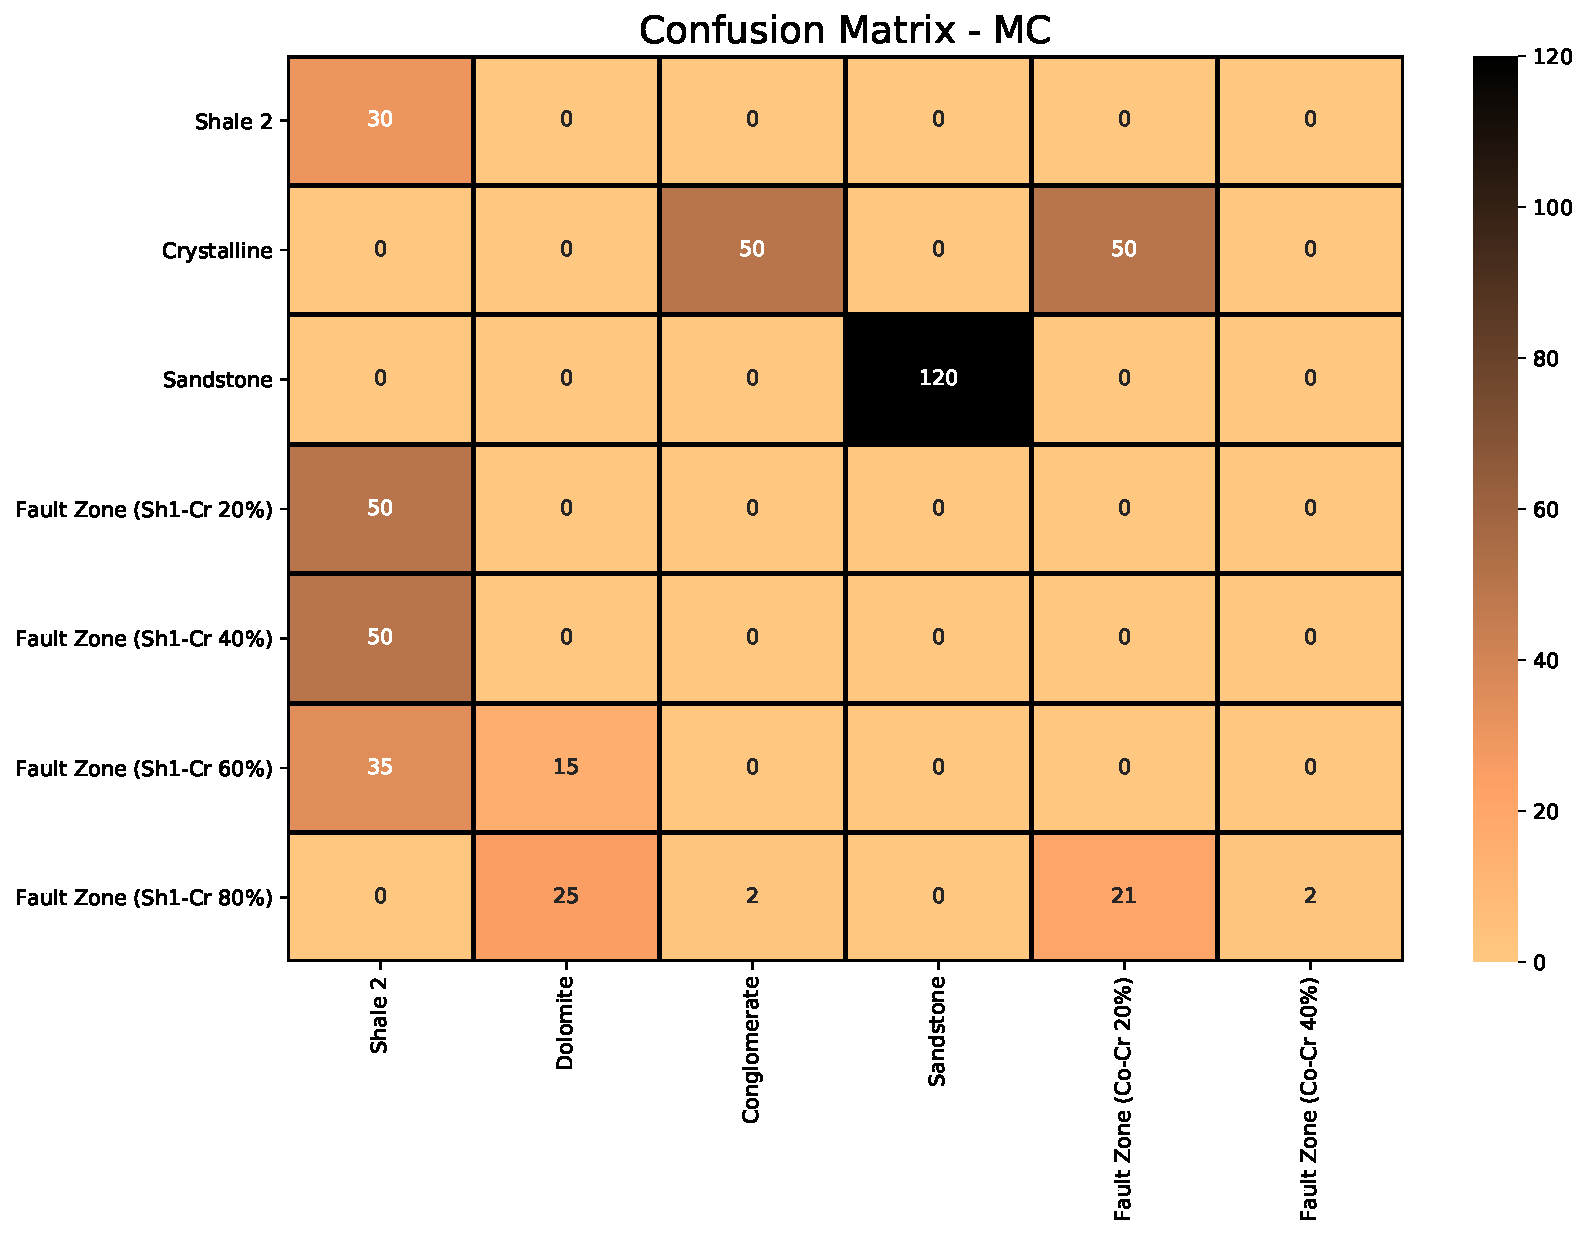
\includegraphics[scale=0.32]{imagens/CM_Maha_C3.pdf}} \\
		\subfloat[]
		{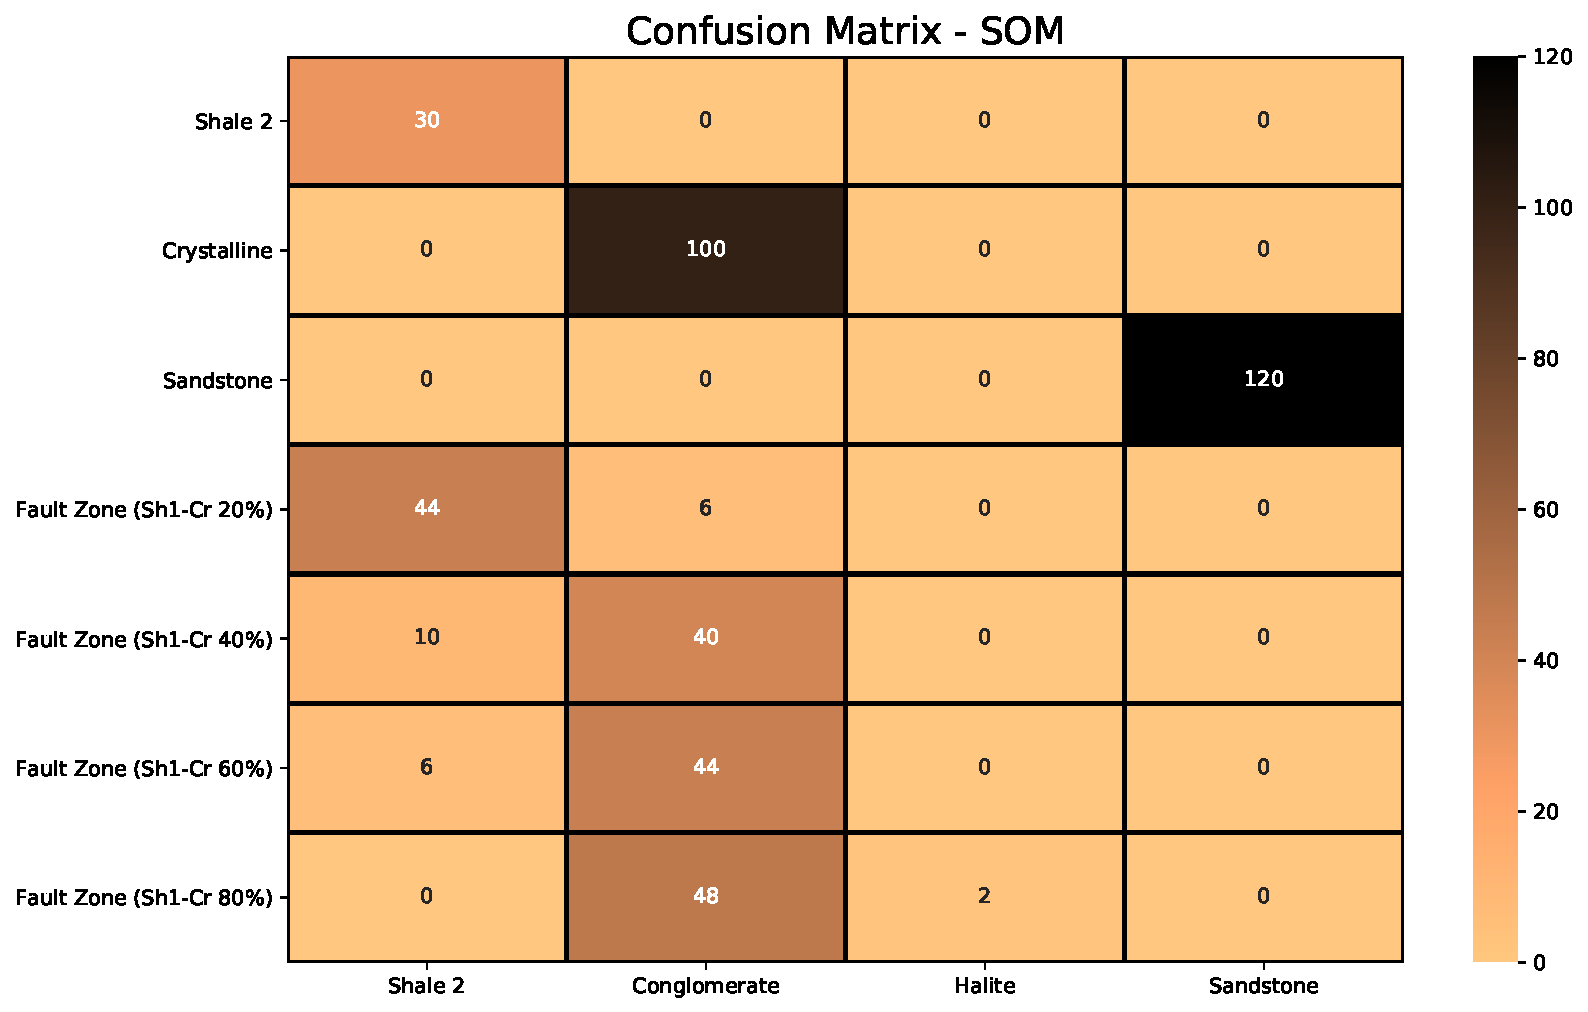
\includegraphics[scale=0.32]{imagens/CM_Kohonen_C3.pdf}} 
		\caption{ Confusion Matrix for (a) Euclidean Classifier , (b) Mahalanobis Classifier and (c) Self-Organizing Map. Colors shows the number of each rock unit comprising well C3.}
		\label{fig:CM_C3}
	\end{center}
\end{figure*}

\section{Results with real log data: Paran\'a Basin}
\label{sub:Real}


%\section{DISCUSSIONS}
%\label{sec:Disc}

\section{Conclusions}
\label{sec:Conc}

\section{Acknowledgments}
\label{sec:Ackn}

%% The Appendices part is started with the command \appendix;
%% appendix sections are then done as normal sections
%% \appendix

%% \section{}
%% \label{}

%% References
%%
%% Following citation commands can be used in the body text:
%% Usage of \cite is as follows:
%%   \cite{key}          ==>>  [#]
%%   \cite[chap. 2]{key} ==>>  [#, chap. 2]
%%   \citet{key}         ==>>  Author [#]

%% References with bibTeX database:

\pagebreak
\bibliographystyle{model2-names.bst}\biboptions{authoryear}
\bibliography{article.bib}

\end{document}
